\documentclass{report}

%%%%%%%%%%%%%%%%%%%%%%%%%%%%%%%%%
% PACKAGE IMPORTS
%%%%%%%%%%%%%%%%%%%%%%%%%%%%%%%%%


% Codificación y tipografía básica (se cargan aquí para orden correcto)
\usepackage[utf8]{inputenc}
\usepackage[T1]{fontenc}
\usepackage{lmodern}
% Idioma español para nombres de elementos flotantes (Figura, Tabla, etc.)
\usepackage[spanish]{babel}
% Asegurar nombre de tablas en español
\addto\captionsspanish{\renewcommand{\tablename}{Tabla}}


\usepackage[tmargin=2cm,rmargin=1in,lmargin=1in,margin=0.85in,bmargin=2cm,footskip=.2in]{geometry}
\usepackage{amsmath,amsfonts,amsthm,amssymb,mathtools}
\usepackage[varbb]{newpxmath}
\usepackage{xfrac}
\usepackage[makeroom]{cancel}
\usepackage{mathtools}
\usepackage{bookmark}
\usepackage{enumitem}
\usepackage{hyperref,theoremref}
\hypersetup{
	pdftitle={Assignment},
	colorlinks=true, linkcolor=gray,citecolor=blue,
	bookmarksnumbered=true,
	bookmarksopen=true
}
\usepackage[most,many,breakable]{tcolorbox}
\usepackage{xcolor}
\usepackage{varwidth}
\usepackage{varwidth}
\usepackage{etoolbox}
%\usepackage{authblk}
\usepackage{nameref}
\usepackage{multicol,array}
\usepackage{tikz-cd}
\usepackage[ruled,vlined,linesnumbered]{algorithm2e}
\usepackage{comment} % enables the use of multi-line comments (\ifx \fi) 
\usepackage{import}
\usepackage{xifthen}
\usepackage{pdfpages}
\usepackage{transparent}

\newcommand\mycommfont[1]{\footnotesize\ttfamily\textcolor{blue}{#1}}
\SetCommentSty{mycommfont}
\newcommand{\incfig}[1]{%
    \def\svgwidth{\columnwidth}
    \import{./figures/}{#1.pdf_tex}
}

\usepackage{tikzsymbols}
\renewcommand\qedsymbol{$\Laughey$}


%\usepackage{import}
%\usepackage{xifthen}
%\usepackage{pdfpages}
%\usepackage{transparent}


%%%%%%%%%%%%%%%%%%%%%%%%%%%%%%
% SELF MADE COLORS
%%%%%%%%%%%%%%%%%%%%%%%%%%%%%%



\definecolor{myg}{RGB}{56, 140, 70}
\definecolor{myb}{RGB}{45, 111, 177}
\definecolor{myr}{RGB}{199, 68, 64}
\definecolor{mytheorembg}{HTML}{F2F2F9}
\definecolor{mytheoremfr}{HTML}{00007B}
\definecolor{mylenmabg}{HTML}{FFFAF8}
\definecolor{mylenmafr}{HTML}{983b0f}
\definecolor{mypropbg}{HTML}{f2fbfc}
\definecolor{mypropfr}{HTML}{191971}
\definecolor{myexamplebg}{HTML}{F2FBF8}
\definecolor{myexamplefr}{HTML}{88D6D1}
\definecolor{myexampleti}{HTML}{2A7F7F}
\definecolor{mydefinitbg}{HTML}{E5E5FF}
\definecolor{mydefinitfr}{HTML}{3F3FA3}
\definecolor{notesgreen}{RGB}{0,162,0}
\definecolor{myp}{RGB}{197, 92, 212}
\definecolor{mygr}{HTML}{2C3338}
\definecolor{myred}{RGB}{127,0,0}
\definecolor{myyellow}{RGB}{169,121,69}
\definecolor{myexercisebg}{HTML}{F2FBF8}
\definecolor{myexercisefg}{HTML}{88D6D1}


%%%%%%%%%%%%%%%%%%%%%%%%%%%%
% TCOLORBOX SETUPS
%%%%%%%%%%%%%%%%%%%%%%%%%%%%

\setlength{\parindent}{1cm}
%================================
% THEOREM BOX
%================================

\tcbuselibrary{theorems,skins,hooks}
\newtcbtheorem[number within=section]{Theorem}{Theorem}
{%
	enhanced,
	breakable,
	colback = mytheorembg,
	frame hidden,
	boxrule = 0sp,
	borderline west = {2pt}{0pt}{mytheoremfr},
	sharp corners,
	detach title,
	before upper = \tcbtitle\par\smallskip,
	coltitle = mytheoremfr,
	fonttitle = \bfseries\sffamily,
	description font = \mdseries,
	separator sign none,
	segmentation style={solid, mytheoremfr},
}
{th}

\tcbuselibrary{theorems,skins,hooks}
\newtcbtheorem[number within=chapter]{theorem}{Theorem}
{%
	enhanced,
	breakable,
	colback = mytheorembg,
	frame hidden,
	boxrule = 0sp,
	borderline west = {2pt}{0pt}{mytheoremfr},
	sharp corners,
	detach title,
	before upper = \tcbtitle\par\smallskip,
	coltitle = mytheoremfr,
	fonttitle = \bfseries\sffamily,
	description font = \mdseries,
	separator sign none,
	segmentation style={solid, mytheoremfr},
}
{th}


\tcbuselibrary{theorems,skins,hooks}
\newtcolorbox{Theoremcon}
{%
	enhanced
	,breakable
	,colback = mytheorembg
	,frame hidden
	,boxrule = 0sp
	,borderline west = {2pt}{0pt}{mytheoremfr}
	,sharp corners
	,description font = \mdseries
	,separator sign none
}

%================================
% Corollery
%================================
\tcbuselibrary{theorems,skins,hooks}
\newtcbtheorem[number within=section]{Corollary}{Corollary}
{%
	enhanced
	,breakable
	,colback = myp!10
	,frame hidden
	,boxrule = 0sp
	,borderline west = {2pt}{0pt}{myp!85!black}
	,sharp corners
	,detach title
	,before upper = \tcbtitle\par\smallskip
	,coltitle = myp!85!black
	,fonttitle = \bfseries\sffamily
	,description font = \mdseries
	,separator sign none
	,segmentation style={solid, myp!85!black}
}
{th}
\tcbuselibrary{theorems,skins,hooks}
\newtcbtheorem[number within=chapter]{corollary}{Corollary}
{%
	enhanced
	,breakable
	,colback = myp!10
	,frame hidden
	,boxrule = 0sp
	,borderline west = {2pt}{0pt}{myp!85!black}
	,sharp corners
	,detach title
	,before upper = \tcbtitle\par\smallskip
	,coltitle = myp!85!black
	,fonttitle = \bfseries\sffamily
	,description font = \mdseries
	,separator sign none
	,segmentation style={solid, myp!85!black}
}
{th}


%================================
% LENMA
%================================

\tcbuselibrary{theorems,skins,hooks}
\newtcbtheorem[number within=section]{Lenma}{Lenma}
{%
	enhanced,
	breakable,
	colback = mylenmabg,
	frame hidden,
	boxrule = 0sp,
	borderline west = {2pt}{0pt}{mylenmafr},
	sharp corners,
	detach title,
	before upper = \tcbtitle\par\smallskip,
	coltitle = mylenmafr,
	fonttitle = \bfseries\sffamily,
	description font = \mdseries,
	separator sign none,
	segmentation style={solid, mylenmafr},
}
{th}

\tcbuselibrary{theorems,skins,hooks}
\newtcbtheorem[number within=chapter]{lenma}{Lenma}
{%
	enhanced,
	breakable,
	colback = mylenmabg,
	frame hidden,
	boxrule = 0sp,
	borderline west = {2pt}{0pt}{mylenmafr},
	sharp corners,
	detach title,
	before upper = \tcbtitle\par\smallskip,
	coltitle = mylenmafr,
	fonttitle = \bfseries\sffamily,
	description font = \mdseries,
	separator sign none,
	segmentation style={solid, mylenmafr},
}
{th}


%================================
% PROPOSITION
%================================

\tcbuselibrary{theorems,skins,hooks}
\newtcbtheorem[number within=section]{Prop}{Proposition}
{%
	enhanced,
	breakable,
	colback = mypropbg,
	frame hidden,
	boxrule = 0sp,
	borderline west = {2pt}{0pt}{mypropfr},
	sharp corners,
	detach title,
	before upper = \tcbtitle\par\smallskip,
	coltitle = mypropfr,
	fonttitle = \bfseries\sffamily,
	description font = \mdseries,
	separator sign none,
	segmentation style={solid, mypropfr},
}
{th}

\tcbuselibrary{theorems,skins,hooks}
\newtcbtheorem[number within=chapter]{prop}{Proposition}
{%
	enhanced,
	breakable,
	colback = mypropbg,
	frame hidden,
	boxrule = 0sp,
	borderline west = {2pt}{0pt}{mypropfr},
	sharp corners,
	detach title,
	before upper = \tcbtitle\par\smallskip,
	coltitle = mypropfr,
	fonttitle = \bfseries\sffamily,
	description font = \mdseries,
	separator sign none,
	segmentation style={solid, mypropfr},
}
{th}


%================================
% CLAIM
%================================

\tcbuselibrary{theorems,skins,hooks}
\newtcbtheorem[number within=section]{claim}{Claim}
{%
	enhanced
	,breakable
	,colback = myg!10
	,frame hidden
	,boxrule = 0sp
	,borderline west = {2pt}{0pt}{myg}
	,sharp corners
	,detach title
	,before upper = \tcbtitle\par\smallskip
	,coltitle = myg!85!black
	,fonttitle = \bfseries\sffamily
	,description font = \mdseries
	,separator sign none
	,segmentation style={solid, myg!85!black}
}
{th}



%================================
% Exercise
%================================

\tcbuselibrary{theorems,skins,hooks}
\newtcbtheorem[number within=section]{Exercise}{Exercise}
{%
	enhanced,
	breakable,
	colback = myexercisebg,
	frame hidden,
	boxrule = 0sp,
	borderline west = {2pt}{0pt}{myexercisefg},
	sharp corners,
	detach title,
	before upper = \tcbtitle\par\smallskip,
	coltitle = myexercisefg,
	fonttitle = \bfseries\sffamily,
	description font = \mdseries,
	separator sign none,
	segmentation style={solid, myexercisefg},
}
{th}

\tcbuselibrary{theorems,skins,hooks}
\newtcbtheorem[number within=chapter]{exercise}{Exercise}
{%
	enhanced,
	breakable,
	colback = myexercisebg,
	frame hidden,
	boxrule = 0sp,
	borderline west = {2pt}{0pt}{myexercisefg},
	sharp corners,
	detach title,
	before upper = \tcbtitle\par\smallskip,
	coltitle = myexercisefg,
	fonttitle = \bfseries\sffamily,
	description font = \mdseries,
	separator sign none,
	segmentation style={solid, myexercisefg},
}
{th}

%================================
% EXAMPLE BOX
%================================

\newtcbtheorem[number within=section]{Example}{Example}
{%
	colback = myexamplebg
	,breakable
	,colframe = myexamplefr
	,coltitle = myexampleti
	,boxrule = 1pt
	,sharp corners
	,detach title
	,before upper=\tcbtitle\par\smallskip
	,fonttitle = \bfseries
	,description font = \mdseries
	,separator sign none
	,description delimiters parenthesis
}
{ex}

\newtcbtheorem[number within=chapter]{example}{Example}
{%
	colback = myexamplebg
	,breakable
	,colframe = myexamplefr
	,coltitle = myexampleti
	,boxrule = 1pt
	,sharp corners
	,detach title
	,before upper=\tcbtitle\par\smallskip
	,fonttitle = \bfseries
	,description font = \mdseries
	,separator sign none
	,description delimiters parenthesis
}
{ex}

%================================
% DEFINITION BOX
%================================

\newtcbtheorem[number within=section]{Definition}{Definition}{enhanced,
	before skip=2mm,after skip=2mm, colback=red!5,colframe=red!80!black,boxrule=0.5mm,
	attach boxed title to top left={xshift=1cm,yshift*=1mm-\tcboxedtitleheight}, varwidth boxed title*=-3cm,
	boxed title style={frame code={
					\path[fill=tcbcolback]
					([yshift=-1mm,xshift=-1mm]frame.north west)
					arc[start angle=0,end angle=180,radius=1mm]
					([yshift=-1mm,xshift=1mm]frame.north east)
					arc[start angle=180,end angle=0,radius=1mm];
					\path[left color=tcbcolback!60!black,right color=tcbcolback!60!black,
						middle color=tcbcolback!80!black]
					([xshift=-2mm]frame.north west) -- ([xshift=2mm]frame.north east)
					[rounded corners=1mm]-- ([xshift=1mm,yshift=-1mm]frame.north east)
					-- (frame.south east) -- (frame.south west)
					-- ([xshift=-1mm,yshift=-1mm]frame.north west)
					[sharp corners]-- cycle;
				},interior engine=empty,
		},
	fonttitle=\bfseries,
	title={#2},#1}{def}
\newtcbtheorem[number within=chapter]{definition}{Definition}{enhanced,
	before skip=2mm,after skip=2mm, colback=red!5,colframe=red!80!black,boxrule=0.5mm,
	attach boxed title to top left={xshift=1cm,yshift*=1mm-\tcboxedtitleheight}, varwidth boxed title*=-3cm,
	boxed title style={frame code={
					\path[fill=tcbcolback]
					([yshift=-1mm,xshift=-1mm]frame.north west)
					arc[start angle=0,end angle=180,radius=1mm]
					([yshift=-1mm,xshift=1mm]frame.north east)
					arc[start angle=180,end angle=0,radius=1mm];
					\path[left color=tcbcolback!60!black,right color=tcbcolback!60!black,
						middle color=tcbcolback!80!black]
					([xshift=-2mm]frame.north west) -- ([xshift=2mm]frame.north east)
					[rounded corners=1mm]-- ([xshift=1mm,yshift=-1mm]frame.north east)
					-- (frame.south east) -- (frame.south west)
					-- ([xshift=-1mm,yshift=-1mm]frame.north west)
					[sharp corners]-- cycle;
				},interior engine=empty,
		},
	fonttitle=\bfseries,
	title={#2},#1}{def}



%================================
% Solution BOX
%================================

\makeatletter
\newtcbtheorem{question}{Pregunta}{enhanced,
	breakable,
	colback=white,
	colframe=myb!80!black,
	attach boxed title to top left={yshift*=-\tcboxedtitleheight},
	fonttitle=\bfseries,
	title={#2},
	boxed title size=title,
	boxed title style={%
			sharp corners,
			rounded corners=northwest,
			colback=tcbcolframe,
			boxrule=0pt,
		},
	underlay boxed title={%
			\path[fill=tcbcolframe] (title.south west)--(title.south east)
			to[out=0, in=180] ([xshift=5mm]title.east)--
			(title.center-|frame.east)
			[rounded corners=\kvtcb@arc] |-
			(frame.north) -| cycle;
		},
	#1
}{def}
\makeatother

%================================
% SOLUTION BOX
%================================

\makeatletter
\newtcolorbox{solution}{enhanced,
	breakable,
	colback=white,
	colframe=myg!80!black,
	attach boxed title to top left={yshift*=-\tcboxedtitleheight},
	title=Solution,
	boxed title size=title,
	boxed title style={%
			sharp corners,
			rounded corners=northwest,
			colback=tcbcolframe,
			boxrule=0pt,
		},
	underlay boxed title={%
			\path[fill=tcbcolframe] (title.south west)--(title.south east)
			to[out=0, in=180] ([xshift=5mm]title.east)--
			(title.center-|frame.east)
			[rounded corners=\kvtcb@arc] |-
			(frame.north) -| cycle;
		},
}
\makeatother

%================================
% Question BOX
%================================

\makeatletter
\newtcbtheorem{qstion}{Pregunta}{enhanced,
	breakable,
	colback=white,
	colframe=mygr,
	attach boxed title to top left={yshift*=-\tcboxedtitleheight},
	fonttitle=\bfseries,
	title={#2},
	boxed title size=title,
	boxed title style={%
			sharp corners,
			rounded corners=northwest,
			colback=tcbcolframe,
			boxrule=0pt,
		},
	underlay boxed title={%
			\path[fill=tcbcolframe] (title.south west)--(title.south east)
			to[out=0, in=180] ([xshift=5mm]title.east)--
			(title.center-|frame.east)
			[rounded corners=\kvtcb@arc] |-
			(frame.north) -| cycle;
		},
	#1
}{def}
\makeatother

\newtcbtheorem[number within=chapter]{wconc}{Wrong Concept}{
	breakable,
	enhanced,
	colback=white,
	colframe=myr,
	arc=0pt,
	outer arc=0pt,
	fonttitle=\bfseries\sffamily\large,
	colbacktitle=myr,
	attach boxed title to top left={},
	boxed title style={
			enhanced,
			skin=enhancedfirst jigsaw,
			arc=3pt,
			bottom=0pt,
			interior style={fill=myr}
		},
	#1
}{def}



%================================
% NOTE BOX
%================================

\usetikzlibrary{arrows,calc,shadows.blur}
\tcbuselibrary{skins}
\newtcolorbox{note}[1][]{%
	enhanced jigsaw,
	colback=gray!20!white,%
	colframe=gray!80!black,
	size=small,
	boxrule=1pt,
	title=\textbf{Nota:-},
	halign title=flush center,
	coltitle=black,
	breakable,
	drop shadow=black!50!white,
	attach boxed title to top left={xshift=1cm,yshift=-\tcboxedtitleheight/2,yshifttext=-\tcboxedtitleheight/2},
	minipage boxed title=1.5cm,
	boxed title style={%
			colback=white,
			size=fbox,
			boxrule=1pt,
			boxsep=2pt,
			underlay={%
					\coordinate (dotA) at ($(interior.west) + (-0.5pt,0)$);
					\coordinate (dotB) at ($(interior.east) + (0.5pt,0)$);
					\begin{scope}
						\clip (interior.north west) rectangle ([xshift=3ex]interior.east);
						\filldraw [white, blur shadow={shadow opacity=60, shadow yshift=-.75ex}, rounded corners=2pt] (interior.north west) rectangle (interior.south east);
					\end{scope}
					\begin{scope}[gray!80!black]
						\fill (dotA) circle (2pt);
						\fill (dotB) circle (2pt);
					\end{scope}
				},
		},
	#1,
}

%%%%%%%%%%%%%%%%%%%%%%%%%%%%%%
% SELF MADE COMMANDS
%%%%%%%%%%%%%%%%%%%%%%%%%%%%%%


\newcommand{\thm}[2]{\begin{Theorem}{#1}{}#2\end{Theorem}}
\newcommand{\cor}[2]{\begin{Corollary}{#1}{}#2\end{Corollary}}
\newcommand{\mlenma}[2]{\begin{Lenma}{#1}{}#2\end{Lenma}}
\newcommand{\mprop}[2]{\begin{Prop}{#1}{}#2\end{Prop}}
\newcommand{\clm}[3]{\begin{claim}{#1}{#2}#3\end{claim}}
\newcommand{\wc}[2]{\begin{wconc}{#1}{}\setlength{\parindent}{1cm}#2\end{wconc}}
\newcommand{\thmcon}[1]{\begin{Theoremcon}{#1}\end{Theoremcon}}
\newcommand{\ex}[2]{\begin{Example}{#1}{}#2\end{Example}}
\newcommand{\dfn}[2]{\begin{Definition}[colbacktitle=red!75!black]{#1}{}#2\end{Definition}}
\newcommand{\dfnc}[2]{\begin{definition}[colbacktitle=red!75!black]{#1}{}#2\end{definition}}
\newcommand{\qs}[2]{\begin{question}{#1}{}#2\end{question}}
\newcommand{\pf}[2]{\begin{myproof}[#1]#2\end{myproof}}
\NewDocumentCommand{\nt}{+m}{\begin{note}#1\end{note}}

\newcommand*\circled[1]{\tikz[baseline=(char.base)]{
		\node[shape=circle,draw,inner sep=1pt] (char) {#1};}}
\newcommand\getcurrentref[1]{%
	\ifnumequal{\value{#1}}{0}
	{??}
	{\the\value{#1}}%
}
\newcommand{\getCurrentSectionNumber}{\getcurrentref{section}}
\newenvironment{myproof}[1][\proofname]{%
	\proof[\bfseries #1: ]%
}{\endproof}

\newcommand{\mclm}[2]{\begin{myclaim}[#1]#2\end{myclaim}}
\newenvironment{myclaim}[1][\claimname]{\proof[\bfseries #1: ]}{}

\newcounter{mylabelcounter}

\makeatletter
\newcommand{\setword}[2]{%
	\phantomsection
	#1\def\@currentlabel{\unexpanded{#1}}\label{#2}%
}
\makeatother




\tikzset{
	symbol/.style={
			draw=none,
			every to/.append style={
					edge node={node [sloped, allow upside down, auto=false]{$#1$}}}
		}
}


% deliminators
\DeclarePairedDelimiter{\abs}{\lvert}{\rvert}
\DeclarePairedDelimiter{\norm}{\lVert}{\rVert}

\DeclarePairedDelimiter{\ceil}{\lceil}{\rceil}
\DeclarePairedDelimiter{\floor}{\lfloor}{\rfloor}
\DeclarePairedDelimiter{\round}{\lfloor}{\rceil}

\newsavebox\diffdbox
\newcommand{\slantedromand}{{\mathpalette\makesl{d}}}
\newcommand{\makesl}[2]{%
\begingroup
\sbox{\diffdbox}{$\mathsurround=0pt#1\mathrm{#2}$}%
\pdfsave
\pdfsetmatrix{1 0 0.2 1}%
\rlap{\usebox{\diffdbox}}%
\pdfrestore
\hskip\wd\diffdbox
\endgroup
}
\newcommand{\dd}[1][]{\ensuremath{\mathop{}\!\ifstrempty{#1}{%
\slantedromand\@ifnextchar^{\hspace{0.2ex}}{\hspace{0.1ex}}}%
{\slantedromand\hspace{0.2ex}^{#1}}}}
\ProvideDocumentCommand\dv{o m g}{%
  \ensuremath{%
    \IfValueTF{#3}{%
      \IfNoValueTF{#1}{%
        \frac{\dd #2}{\dd #3}%
      }{%
        \frac{\dd^{#1} #2}{\dd #3^{#1}}%
      }%
    }{%
      \IfNoValueTF{#1}{%
        \frac{\dd}{\dd #2}%
      }{%
        \frac{\dd^{#1}}{\dd #2^{#1}}%
      }%
    }%
  }%
}
\providecommand*{\pdv}[3][]{\frac{\partial^{#1}#2}{\partial#3^{#1}}}
%  - others
\DeclareMathOperator{\Lap}{\mathcal{L}}
\DeclareMathOperator{\Var}{Var} % varience
\DeclareMathOperator{\Cov}{Cov} % covarience
\DeclareMathOperator{\E}{E} % expected

% Since the amsthm package isn't loaded

% I prefer the slanted \leq
\let\oldleq\leq % save them in case they're every wanted
\let\oldgeq\geq
\renewcommand{\leq}{\leqslant}
\renewcommand{\geq}{\geqslant}

% % redefine matrix env to allow for alignment, use r as default
% \renewcommand*\env@matrix[1][r]{\hskip -\arraycolsep
%     \let\@ifnextchar\new@ifnextchar
%     \array{*\c@MaxMatrixCols #1}}


%\usepackage{framed}
%\usepackage{titletoc}
%\usepackage{etoolbox}
%\usepackage{lmodern}


%\patchcmd{\tableofcontents}{\contentsname}{\sffamily\contentsname}{}{}

%\renewenvironment{leftbar}
%{\def\FrameCommand{\hspace{6em}%
%		{\color{myyellow}\vrule width 2pt depth 6pt}\hspace{1em}}%
%	\MakeFramed{\parshape 1 0cm \dimexpr\textwidth-6em\relax\FrameRestore}\vskip2pt%
%}
%{\endMakeFramed}

%\titlecontents{chapter}
%[0em]{\vspace*{2\baselineskip}}
%{\parbox{4.5em}{%
%		\hfill\Huge\sffamily\bfseries\color{myred}\thecontentspage}%
%	\vspace*{-2.3\baselineskip}\leftbar\textsc{\small\chaptername~\thecontentslabel}\\\sffamily}
%{}{\endleftbar}
%\titlecontents{section}
%[8.4em]
%{\sffamily\contentslabel{3em}}{}{}
%{\hspace{0.5em}\nobreak\itshape\color{myred}\contentspage}
%\titlecontents{subsection}
%[8.4em]
%{\sffamily\contentslabel{3em}}{}{}  
%{\hspace{0.5em}\nobreak\itshape\color{myred}\contentspage}



%%%%%%%%%%%%%%%%%%%%%%%%%%%%%%%%%%%%%%%%%%%
% TABLE OF CONTENTS
%%%%%%%%%%%%%%%%%%%%%%%%%%%%%%%%%%%%%%%%%%%

\usepackage{tikz}
\definecolor{doc}{RGB}{0,60,110}
\usepackage{titletoc}
\contentsmargin{0cm}
\titlecontents{chapter}[3.7pc]
{\addvspace{30pt}%
	\begin{tikzpicture}[remember picture, overlay]%
		\draw[fill=doc!60,draw=doc!60] (-7,-.1) rectangle (-0.9,.5);%
		\pgftext[left,x=-3.5cm,y=0.2cm]{\color{white}\Large\sc\bfseries Módulo\ \thecontentslabel};%
	\end{tikzpicture}\color{doc!60}\large\sc\bfseries}%
{}
{}
{\;\titlerule\;\large\sc\bfseries Page \thecontentspage
	\begin{tikzpicture}[remember picture, overlay]
		\draw[fill=doc!60,draw=doc!60] (2pt,0) rectangle (4,0.1pt);
	\end{tikzpicture}}%
\titlecontents{section}[3.7pc]
{\addvspace{2pt}}
{\contentslabel[\thecontentslabel]{2pc}}
{}
{\hfill\small \thecontentspage}
[]

\titlecontents*{subsection}[4.7pc] % Mayor indentación para subsecciones
{\addvspace{1pt}\small} % Espaciado más limpio
{\thecontentslabel\quad} % Mostrar número de subsección (1.1.1, 1.1.2)
{}
{\hfill\small\thecontentspage\\} % Alinear el número de página correctamente


\makeatletter
\renewcommand{\tableofcontents}{%
	\chapter*{%
	  \vspace*{-20\p@}%
	  \begin{tikzpicture}[remember picture, overlay]%
		  \pgftext[right,x=15cm,y=0.2cm]{\color{doc!60}\Huge\sc\bfseries \contentsname};%
		  \draw[fill=doc!60,draw=doc!60] (13.5,-.75) rectangle (20,1);%
		  \clip (13.4,-.75) rectangle (20,1);
		  \pgftext[right,x=15cm,y=0.2cm]{\color{white}\Huge\sc\bfseries \contentsname};%
	  \end{tikzpicture}}%
	\@starttoc{toc}}
\makeatother

 % Configuración y paquetes de diseño
%From M275 "Topology" at SJSU
\newcommand{\id}{\mathrm{id}}
\newcommand{\taking}[1]{\xrightarrow{#1}}
\newcommand{\inv}{^{-1}}

%From M170 "Introduction to Graph Theory" at SJSU
\DeclareMathOperator{\diam}{diam}
\DeclareMathOperator{\ord}{ord}
\newcommand{\defeq}{\overset{\mathrm{def}}{=}}

%From the USAMO .tex files
\newcommand{\ts}{\textsuperscript}
\newcommand{\dg}{^\circ}
\newcommand{\ii}{\item}

% % From Math 55 and Math 145 at Harvard
% \newenvironment{subproof}[1][Proof]{%
% \begin{proof}[#1] \renewcommand{\qedsymbol}{$\blacksquare$}}%
% {\end{proof}}

\newcommand{\liff}{\leftrightarrow}
\newcommand{\lthen}{\rightarrow}
\newcommand{\opname}{\operatorname}
\newcommand{\surjto}{\twoheadrightarrow}
\newcommand{\injto}{\hookrightarrow}
\newcommand{\On}{\mathrm{On}} % ordinals
\DeclareMathOperator{\img}{im} % Image
\DeclareMathOperator{\Img}{Im} % Image
\DeclareMathOperator{\coker}{coker} % Cokernel
\DeclareMathOperator{\Coker}{Coker} % Cokernel
\DeclareMathOperator{\Ker}{Ker} % Kernel
\DeclareMathOperator{\rank}{rank}
\DeclareMathOperator{\Spec}{Spec} % spectrum
\DeclareMathOperator{\Tr}{Tr} % trace
\DeclareMathOperator{\pr}{pr} % projection
\DeclareMathOperator{\ext}{ext} % extension
\DeclareMathOperator{\pred}{pred} % predecessor
\DeclareMathOperator{\dom}{dom} % domain
\DeclareMathOperator{\ran}{ran} % range
\DeclareMathOperator{\Hom}{Hom} % homomorphism
\DeclareMathOperator{\Mor}{Mor} % morphisms
\DeclareMathOperator{\End}{End} % endomorphism

\newcommand{\eps}{\epsilon}
\newcommand{\veps}{\varepsilon}
\newcommand{\ol}{\overline}
\newcommand{\ul}{\underline}
\newcommand{\wt}{\widetilde}
\newcommand{\wh}{\widehat}
\newcommand{\vocab}[1]{\textbf{\color{blue} #1}}
\providecommand{\half}{\frac{1}{2}}
\newcommand{\dang}{\measuredangle} %% Directed angle
\newcommand{\ray}[1]{\overrightarrow{#1}}
\newcommand{\seg}[1]{\overline{#1}}
\newcommand{\arc}[1]{\wideparen{#1}}
\DeclareMathOperator{\cis}{cis}
\DeclareMathOperator*{\lcm}{lcm}
\DeclareMathOperator*{\argmin}{arg min}
\DeclareMathOperator*{\argmax}{arg max}
\newcommand{\cycsum}{\sum_{\mathrm{cyc}}}
\newcommand{\symsum}{\sum_{\mathrm{sym}}}
\newcommand{\cycprod}{\prod_{\mathrm{cyc}}}
\newcommand{\symprod}{\prod_{\mathrm{sym}}}
\newcommand{\Qed}{\begin{flushright}\qed\end{flushright}}
\newcommand{\parinn}{\setlength{\parindent}{1cm}}
\newcommand{\parinf}{\setlength{\parindent}{0cm}}
% \newcommand{\norm}{\|\cdot\|}
\newcommand{\inorm}{\norm_{\infty}}
\newcommand{\opensets}{\{V_{\alpha}\}_{\alpha\in I}}
\newcommand{\oset}{V_{\alpha}}
\newcommand{\opset}[1]{V_{\alpha_{#1}}}
\newcommand{\lub}{\text{lub}}
\newcommand{\del}[2]{\frac{\partial #1}{\partial #2}}
\newcommand{\Del}[3]{\frac{\partial^{#1} #2}{\partial^{#1} #3}}
\newcommand{\deld}[2]{\dfrac{\partial #1}{\partial #2}}
\newcommand{\Deld}[3]{\dfrac{\partial^{#1} #2}{\partial^{#1} #3}}
\newcommand{\lm}{\lambda}
\newcommand{\uin}{\mathbin{\rotatebox[origin=c]{90}{$\in$}}}
\newcommand{\usubset}{\mathbin{\rotatebox[origin=c]{90}{$\subset$}}}
\newcommand{\lt}{\left}
\newcommand{\rt}{\right}
\newcommand{\bs}[1]{\boldsymbol{#1}}
\newcommand{\exs}{\exists}
\newcommand{\st}{\strut}
\newcommand{\dps}[1]{\displaystyle{#1}}

\newcommand{\sol}{\setlength{\parindent}{0cm}\textbf{\textit{Solution:}}\setlength{\parindent}{1cm} }
\newcommand{\solve}[1]{\setlength{\parindent}{0cm}\textbf{\textit{Solución: }}\setlength{\parindent}{1cm}#1 \Qed}

% Things Lie
\newcommand{\kb}{\mathfrak b}
\newcommand{\kg}{\mathfrak g}
\newcommand{\kh}{\mathfrak h}
\newcommand{\kn}{\mathfrak n}
\newcommand{\ku}{\mathfrak u}
\newcommand{\kz}{\mathfrak z}
\DeclareMathOperator{\Ext}{Ext} % Ext functor
\DeclareMathOperator{\Tor}{Tor} % Tor functor
\newcommand{\gl}{\opname{\mathfrak{gl}}} % frak gl group
\renewcommand{\sl}{\opname{\mathfrak{sl}}} % frak sl group chktex 6

% More script letters etc.
\newcommand{\SA}{\mathcal A}
\newcommand{\SB}{\mathcal B}
\newcommand{\SC}{\mathcal C}
\newcommand{\SF}{\mathcal F}
\newcommand{\SG}{\mathcal G}
\newcommand{\SH}{\mathcal H}
\newcommand{\OO}{\mathcal O}

\newcommand{\SCA}{\mathscr A}
\newcommand{\SCB}{\mathscr B}
\newcommand{\SCC}{\mathscr C}
\newcommand{\SCD}{\mathscr D}
\newcommand{\SCE}{\mathscr E}
\newcommand{\SCF}{\mathscr F}
\newcommand{\SCG}{\mathscr G}
\newcommand{\SCH}{\mathscr H}

% Mathfrak primes
\newcommand{\km}{\mathfrak m}
\newcommand{\kp}{\mathfrak p}
\newcommand{\kq}{\mathfrak q}

% number sets
\newcommand{\RR}[1][]{\ensuremath{\ifstrempty{#1}{\mathbb{R}}{\mathbb{R}^{#1}}}}
\newcommand{\NN}[1][]{\ensuremath{\ifstrempty{#1}{\mathbb{N}}{\mathbb{N}^{#1}}}}
\newcommand{\ZZ}[1][]{\ensuremath{\ifstrempty{#1}{\mathbb{Z}}{\mathbb{Z}^{#1}}}}
\newcommand{\QQ}[1][]{\ensuremath{\ifstrempty{#1}{\mathbb{Q}}{\mathbb{Q}^{#1}}}}
\newcommand{\CC}[1][]{\ensuremath{\ifstrempty{#1}{\mathbb{C}}{\mathbb{C}^{#1}}}}
\newcommand{\PP}[1][]{\ensuremath{\ifstrempty{#1}{\mathbb{P}}{\mathbb{P}^{#1}}}}
\newcommand{\HH}[1][]{\ensuremath{\ifstrempty{#1}{\mathbb{H}}{\mathbb{H}^{#1}}}}
\newcommand{\FF}[1][]{\ensuremath{\ifstrempty{#1}{\mathbb{F}}{\mathbb{F}^{#1}}}}
% expected value
\newcommand{\EE}{\ensuremath{\mathbb{E}}}
\newcommand{\charin}{\text{ char }}
\DeclareMathOperator{\sign}{sign}
\DeclareMathOperator{\Aut}{Aut}
\DeclareMathOperator{\Inn}{Inn}
\DeclareMathOperator{\Syl}{Syl}
\DeclareMathOperator{\Gal}{Gal}
\DeclareMathOperator{\GL}{GL} % General linear group
\DeclareMathOperator{\SL}{SL} % Special linear group

%---------------------------------------
% BlackBoard Math Fonts :-
%---------------------------------------

%Captital Letters
\newcommand{\bbA}{\mathbb{A}}	\newcommand{\bbB}{\mathbb{B}}
\newcommand{\bbC}{\mathbb{C}}	\newcommand{\bbD}{\mathbb{D}}
\newcommand{\bbE}{\mathbb{E}}	\newcommand{\bbF}{\mathbb{F}}
\newcommand{\bbG}{\mathbb{G}}	\newcommand{\bbH}{\mathbb{H}}
\newcommand{\bbI}{\mathbb{I}}	\newcommand{\bbJ}{\mathbb{J}}
\newcommand{\bbK}{\mathbb{K}}	\newcommand{\bbL}{\mathbb{L}}
\newcommand{\bbM}{\mathbb{M}}	\newcommand{\bbN}{\mathbb{N}}
\newcommand{\bbO}{\mathbb{O}}	\newcommand{\bbP}{\mathbb{P}}
\newcommand{\bbQ}{\mathbb{Q}}	\newcommand{\bbR}{\mathbb{R}}
\newcommand{\bbS}{\mathbb{S}}	\newcommand{\bbT}{\mathbb{T}}
\newcommand{\bbU}{\mathbb{U}}	\newcommand{\bbV}{\mathbb{V}}
\newcommand{\bbW}{\mathbb{W}}	\newcommand{\bbX}{\mathbb{X}}
\newcommand{\bbY}{\mathbb{Y}}	\newcommand{\bbZ}{\mathbb{Z}}

%---------------------------------------
% MathCal Fonts :-
%---------------------------------------

%Captital Letters
\newcommand{\mcA}{\mathcal{A}}	\newcommand{\mcB}{\mathcal{B}}
\newcommand{\mcC}{\mathcal{C}}	\newcommand{\mcD}{\mathcal{D}}
\newcommand{\mcE}{\mathcal{E}}	\newcommand{\mcF}{\mathcal{F}}
\newcommand{\mcG}{\mathcal{G}}	\newcommand{\mcH}{\mathcal{H}}
\newcommand{\mcI}{\mathcal{I}}	\newcommand{\mcJ}{\mathcal{J}}
\newcommand{\mcK}{\mathcal{K}}	\newcommand{\mcL}{\mathcal{L}}
\newcommand{\mcM}{\mathcal{M}}	\newcommand{\mcN}{\mathcal{N}}
\newcommand{\mcO}{\mathcal{O}}	\newcommand{\mcP}{\mathcal{P}}
\newcommand{\mcQ}{\mathcal{Q}}	\newcommand{\mcR}{\mathcal{R}}
\newcommand{\mcS}{\mathcal{S}}	\newcommand{\mcT}{\mathcal{T}}
\newcommand{\mcU}{\mathcal{U}}	\newcommand{\mcV}{\mathcal{V}}
\newcommand{\mcW}{\mathcal{W}}	\newcommand{\mcX}{\mathcal{X}}
\newcommand{\mcY}{\mathcal{Y}}	\newcommand{\mcZ}{\mathcal{Z}}


%---------------------------------------
% Bold Math Fonts :-
%---------------------------------------

%Captital Letters
\newcommand{\bmA}{\boldsymbol{A}}	\newcommand{\bmB}{\boldsymbol{B}}
\newcommand{\bmC}{\boldsymbol{C}}	\newcommand{\bmD}{\boldsymbol{D}}
\newcommand{\bmE}{\boldsymbol{E}}	\newcommand{\bmF}{\boldsymbol{F}}
\newcommand{\bmG}{\boldsymbol{G}}	\newcommand{\bmH}{\boldsymbol{H}}
\newcommand{\bmI}{\boldsymbol{I}}	\newcommand{\bmJ}{\boldsymbol{J}}
\newcommand{\bmK}{\boldsymbol{K}}	\newcommand{\bmL}{\boldsymbol{L}}
\newcommand{\bmM}{\boldsymbol{M}}	\newcommand{\bmN}{\boldsymbol{N}}
\newcommand{\bmO}{\boldsymbol{O}}	\newcommand{\bmP}{\boldsymbol{P}}
\newcommand{\bmQ}{\boldsymbol{Q}}	\newcommand{\bmR}{\boldsymbol{R}}
\newcommand{\bmS}{\boldsymbol{S}}	\newcommand{\bmT}{\boldsymbol{T}}
\newcommand{\bmU}{\boldsymbol{U}}	\newcommand{\bmV}{\boldsymbol{V}}
\newcommand{\bmW}{\boldsymbol{W}}	\newcommand{\bmX}{\boldsymbol{X}}
\newcommand{\bmY}{\boldsymbol{Y}}	\newcommand{\bmZ}{\boldsymbol{Z}}
%Small Letters
\newcommand{\bma}{\boldsymbol{a}}	\newcommand{\bmb}{\boldsymbol{b}}
\newcommand{\bmc}{\boldsymbol{c}}	\newcommand{\bmd}{\boldsymbol{d}}
\newcommand{\bme}{\boldsymbol{e}}	\newcommand{\bmf}{\boldsymbol{f}}
\newcommand{\bmg}{\boldsymbol{g}}	\newcommand{\bmh}{\boldsymbol{h}}
\newcommand{\bmi}{\boldsymbol{i}}	\newcommand{\bmj}{\boldsymbol{j}}
\newcommand{\bmk}{\boldsymbol{k}}	\newcommand{\bml}{\boldsymbol{l}}
\newcommand{\bmm}{\boldsymbol{m}}	\newcommand{\bmn}{\boldsymbol{n}}
\newcommand{\bmo}{\boldsymbol{o}}	\newcommand{\bmp}{\boldsymbol{p}}
\newcommand{\bmq}{\boldsymbol{q}}	\newcommand{\bmr}{\boldsymbol{r}}
\newcommand{\bms}{\boldsymbol{s}}	\newcommand{\bmt}{\boldsymbol{t}}
\newcommand{\bmu}{\boldsymbol{u}}	\newcommand{\bmv}{\boldsymbol{v}}
\newcommand{\bmw}{\boldsymbol{w}}	\newcommand{\bmx}{\boldsymbol{x}}
\newcommand{\bmy}{\boldsymbol{y}}	\newcommand{\bmz}{\boldsymbol{z}}

%---------------------------------------
% Scr Math Fonts :-
%---------------------------------------

\newcommand{\sA}{{\mathscr{A}}}   \newcommand{\sB}{{\mathscr{B}}}
\newcommand{\sC}{{\mathscr{C}}}   \newcommand{\sD}{{\mathscr{D}}}
\newcommand{\sE}{{\mathscr{E}}}   \newcommand{\sF}{{\mathscr{F}}}
\newcommand{\sG}{{\mathscr{G}}}   \newcommand{\sH}{{\mathscr{H}}}
\newcommand{\sI}{{\mathscr{I}}}   \newcommand{\sJ}{{\mathscr{J}}}
\newcommand{\sK}{{\mathscr{K}}}   \newcommand{\sL}{{\mathscr{L}}}
\newcommand{\sM}{{\mathscr{M}}}   \newcommand{\sN}{{\mathscr{N}}}
\newcommand{\sO}{{\mathscr{O}}}   \newcommand{\sP}{{\mathscr{P}}}
\newcommand{\sQ}{{\mathscr{Q}}}   \newcommand{\sR}{{\mathscr{R}}}
\newcommand{\sS}{{\mathscr{S}}}   \newcommand{\sT}{{\mathscr{T}}}
\newcommand{\sU}{{\mathscr{U}}}   \newcommand{\sV}{{\mathscr{V}}}
\newcommand{\sW}{{\mathscr{W}}}   \newcommand{\sX}{{\mathscr{X}}}
\newcommand{\sY}{{\mathscr{Y}}}   \newcommand{\sZ}{{\mathscr{Z}}}


%---------------------------------------
% Math Fraktur Font
%---------------------------------------

%Captital Letters
\newcommand{\mfA}{\mathfrak{A}}	\newcommand{\mfB}{\mathfrak{B}}
\newcommand{\mfC}{\mathfrak{C}}	\newcommand{\mfD}{\mathfrak{D}}
\newcommand{\mfE}{\mathfrak{E}}	\newcommand{\mfF}{\mathfrak{F}}
\newcommand{\mfG}{\mathfrak{G}}	\newcommand{\mfH}{\mathfrak{H}}
\newcommand{\mfI}{\mathfrak{I}}	\newcommand{\mfJ}{\mathfrak{J}}
\newcommand{\mfK}{\mathfrak{K}}	\newcommand{\mfL}{\mathfrak{L}}
\newcommand{\mfM}{\mathfrak{M}}	\newcommand{\mfN}{\mathfrak{N}}
\newcommand{\mfO}{\mathfrak{O}}	\newcommand{\mfP}{\mathfrak{P}}
\newcommand{\mfQ}{\mathfrak{Q}}	\newcommand{\mfR}{\mathfrak{R}}
\newcommand{\mfS}{\mathfrak{S}}	\newcommand{\mfT}{\mathfrak{T}}
\newcommand{\mfU}{\mathfrak{U}}	\newcommand{\mfV}{\mathfrak{V}}
\newcommand{\mfW}{\mathfrak{W}}	\newcommand{\mfX}{\mathfrak{X}}
\newcommand{\mfY}{\mathfrak{Y}}	\newcommand{\mfZ}{\mathfrak{Z}}
%Small Letters
\newcommand{\mfa}{\mathfrak{a}}	\newcommand{\mfb}{\mathfrak{b}}
\newcommand{\mfc}{\mathfrak{c}}	\newcommand{\mfd}{\mathfrak{d}}
\newcommand{\mfe}{\mathfrak{e}}	\newcommand{\mff}{\mathfrak{f}}
\newcommand{\mfg}{\mathfrak{g}}	\newcommand{\mfh}{\mathfrak{h}}
\newcommand{\mfi}{\mathfrak{i}}	\newcommand{\mfj}{\mathfrak{j}}
\newcommand{\mfk}{\mathfrak{k}}	\newcommand{\mfl}{\mathfrak{l}}
\newcommand{\mfm}{\mathfrak{m}}	\newcommand{\mfn}{\mathfrak{n}}
\newcommand{\mfo}{\mathfrak{o}}	\newcommand{\mfp}{\mathfrak{p}}
\newcommand{\mfq}{\mathfrak{q}}	\newcommand{\mfr}{\mathfrak{r}}
\newcommand{\mfs}{\mathfrak{s}}	\newcommand{\mft}{\mathfrak{t}}
\newcommand{\mfu}{\mathfrak{u}}	\newcommand{\mfv}{\mathfrak{v}}
\newcommand{\mfw}{\mathfrak{w}}	\newcommand{\mfx}{\mathfrak{x}}
\newcommand{\mfy}{\mathfrak{y}}	\newcommand{\mfz}{\mathfrak{z}}


\usepackage{booktabs}
\usepackage{siunitx}
\usepackage{adjustbox}
\usepackage{pdflscape}
\usepackage[backend=biber, style=apa]{biblatex}
\usepackage{caption}
\usepackage{multirow}
\usepackage{csquotes}
\usepackage{subcaption}
\usepackage{float}
\usepackage{pgfplots}
\pgfplotsset{compat=1.18}
\usetikzlibrary{positioning, arrows.meta, calc}

\addto\captionsspanish{
  \renewcommand{\contentsname}{Índice General}
}

\graphicspath{ {./Doc/Fotos/} {./figuras/} {./} }
\addbibresource{Referencias.bib}

\definecolor{darkgreen}{rgb}{0,0.6,0}
\definecolor{oliveg}{RGB}{72,118,41}
\definecolor{stoneb}{RGB}{140,86,38}
\definecolor{woodc}{RGB}{43,92,143}

\title{
    
\includegraphics[width=0.32\textwidth]{escudo.png}\\[1.4cm]
    {\LARGE\textbf{Biorrefinería Oleícola por Vía Enzimática y Organosolv}}\\[1.1em]
    {\Large\textbf{Documento nº 2: Estudio de Localización, Implantación y Planos Justificativos}}\\[1.5em]
    {\large\textit{Asignatura: Organización y Gestión de Proyectos --- Curso Académico 2026/2027}}
}
\author{\Large\textbf{Christian Pérez Hita}\\[0.5em] \large Grado en Ingeniería Química \\ \large Escuela Técnica Superior de Ingenierías Informática y de Telecomunicación / Facultad de Ciencias \\ \large Universidad de Granada (UGR)}
\date{Noviembre 2026}

\begin{document}

\maketitle

\begin{abstract}
El presente documento constituye la memoria técnica del estudio de localización e implantación industrial para la implantación de una planta biorrefinería oleícola multibiomasa de escala comercial (\SI{120000}{\tonne\text{ b.s.}/a\text{\~{n}}o}), diseñada para valorizar secuencialmente hueso de aceituna (\SI{15000}{\tonne\text{ b.s.}/a\text{\~{n}}o}), hoja de olivo (\SI{40000}{\tonne\text{ b.s.}/a\text{\~{n}}o}) y madera procedente de restos de poda del olivar (\SI{65000}{\tonne\text{ b.s.}/a\text{\~{n}}o}) mediante fraccionamiento Organosolv e hidrólisis enzimática.

A partir de los aforos oleícolas oficiales de la Agencia de Información y Control Alimentarios (\textcite{AICA2026}) y la base de datos empresarial SABI (\textcite{SABI2026}), se establece como cuenca de captación óptima el triángulo geográfico Córdoba--Granada--Jaén (\num{620} almazaras activas y \num{3885605.3}~t de aceituna molturada en la campaña 2025/2026). La aplicación del método comarcal del \textit{Ratio SABI de Oportunidad} (ingresos de almazaras frente a competencia de plantas de combustión térmica) y el método cualitativo por factores ponderados a nivel macro determina que la provincia de Granada obtiene la máxima puntuación (\num{8.60}/10), superando a Córdoba (\num{8.10}/10) y Jaén (\num{7.45}/10), al presentar la mayor disponibilidad excedentaria de subproductos con mínima canibalización de precios.

A nivel de microlocalización, se contrastan tres alternativas en suelo industrial consolidado: el Polígono Industrial El Manzanil~II en Loja (Granada), el Polígono Industrial Los Santos en Lucena (Córdoba) y el Polígono Industrial Llano Mazuelos en Alcalá la Real (Jaén). El análisis cuantitativo mediante el método de Brown y Gibson, integrando factores críticos ($FC_i = 1$), costes anuales objetivos ($FO_i$) y factores subjetivos ($FS_i$), confirma a Loja como el emplazamiento idóneo con un índice de preferencia $MPL = \num{0.3592}$ (frente a \num{0.3389} en Lucena y \num{0.3019} en Alcalá la Real para $\alpha = \num{0.70}$). El análisis de sensibilidad paramétrico demuestra que Loja es la alternativa dominante de forma incondicional para cualquier valor del factor de ponderación objetiva $\alpha \in [0, 1]$.

El estudio se complementa con la definición de los planos justificativos de situación territorial (escala normalizada 1:50.000 con enlace directo a la autovía A-92) y de localización en parcela (escala 1:2.000, Parcela I-14/15 con \SI{25000}{\square\metre} de superficie neta), la acreditación del cumplimiento estricto del planeamiento urbanístico del PGOU de Loja, la verificación de mano de obra comarcal según el INE, y la formulación de las bases de implantación y ordenación espacial mediante la metodología SLP (\textit{Systematic Layout Planning}) de Muther.
\end{abstract}

\tableofcontents
\newpage

%=============================================================================
\chapter{Introducción, Objeto y Vinculación con el Estudio de Mercado}

\section{Objeto y Alcance del Estudio}
La localización de una planta de proceso químico constituye una de las decisiones estratégicas de mayor trascendencia en la ingeniería de proyectos, condicionando de manera irreversible los costes logísticos de aprovisionamiento de materias primas, los gastos de distribución de productos terminados, el régimen fiscal y normativo aplicable, la disponibilidad de mano de obra cualificada y la viabilidad económica global de la inversión a lo largo de sus \num{20} años de vida útil proyectada.

El presente estudio tiene por objeto determinar, justificar documentalmente y representar cartográficamente el emplazamiento óptimo para la construcción de una planta biorrefinería oleícola, siguiendo los requerimientos metodológicos establecidos en el Seminario de Localización de la asignatura \textit{Organización y Gestión de Proyectos} y las directrices técnicas del Trabajo de Fin de Grado en Ingeniería Química por la Universidad de Granada.

\section{Bases de Capacidad Derivadas del Estudio de Mercado}
Los parámetros de partida dimensionales y cuantitativos se fundamentan estrictamente en los resultados consolidados en el \textit{Estudio de Mercado, Estacionalidad y Capacidad} (Documento nº~1, \textcite{PerezHita2026}):
\begin{enumerate}
    \item \textbf{Capacidad nominal de diseño:} Se adopta el escenario multibiomasa B-5 adaptado con una capacidad global de procesamiento de:
          \begin{equation}
              C_{\text{nominal}} = \SI{120000}{\tonne\text{ b.s.}/a\text{\~{n}}o}
          \end{equation}
          equivalente a un caudal horario de procesamiento continuo de \SI{17.30}{\tonne\text{ b.s.}/h} sobre un régimen de operación industrial de \SI{6936}{h/a\text{\~{n}}o} (\num{289} días hábiles anuales en tres turnos rotativos).
    \item \textbf{Cesta de materias primas lignocelulósicas:}
          \begin{itemize}
              \item \textbf{Hueso de aceituna (\textit{Olive stone}, fracción B-1):} \SI{15000}{\tonne\text{ b.s.}/a\text{\~{n}}o} (\SI{16304}{\tonne/a\text{\~{n}}o} comerciales en base húmeda al \SI{8.0}{\percent}). Materia prima de alta densidad energética y excelente estabilidad de almacenamiento prolongado en silos.
              \item \textbf{Hoja de olivo de almazara y poda (\textit{Olive tree leaves}, fracción B-2):} \SI{40000}{\tonne\text{ b.s.}/a\text{\~{n}}o} (\SI{50000}{\tonne/a\text{\~{n}}o} húmedas al \SI{20.0}{\percent}). Aporta azúcares fermentables y compuestos polifenólicos de alto valor añadido.
              \item \textbf{Madera y ramas de poda del olivar (\textit{Olive tree pruning wood}, fracción B-4):} \SI{65000}{\tonne\text{ b.s.}/a\text{\~{n}}o} (\SI{81250}{\tonne/a\text{\~{n}}o} frescas al \SI{20.0}{\percent}). Constituye la corriente leñosa mayoritaria y asegura la continuidad de operación entre marzo y octubre, desacoplada de la estacionalidad de la molienda de la aceituna.
          \end{itemize}
    \item \textbf{Cuenca de aprovisionamiento de referencia:} El triángulo provincial \textbf{Córdoba--Granada--Jaén}, que agrupa el \SI{55.48}{\percent} de la aceituna molturada en España (\num{3885605.3}~t en \num{620} almazaras activas en la campaña 2025/2026 según \textcite{AICA2026}), generando \num{339602}~t b.s./año de hueso comercial, \num{311038}~t b.s./año de hoja aprovechable y \num{1555763}~t b.s./año de poda de olivo (\num{583411}~t b.s./año de madera gruesa mecanizable).
    \item \textbf{Tasa de captación del proyecto:} El consumo de la planta representa únicamente el \textbf{\SI{4.42}{\percent}} del hueso disponible en el triángulo, el \textbf{\SI{12.86}{\percent}} del potencial foliar y el \textbf{\SI{11.14}{\percent}} de la madera de poda gruesa, lo que garantiza la ausencia absoluta de tensionamiento o desabastecimiento en el mercado comarcal.
\end{enumerate}

\section{Metodología Secuencial de Decisión}
Conforme a las recomendaciones de la literatura especializada en ingeniería de plantas químicas (\textcite{PetersTimmerhaus2003, Turton2018}) y al temario oficial del seminario, el proceso de selección se articula en tres etapas jerárquicas:
\begin{enumerate}
    \item \textbf{Macrolocalización regional:} Selección de la comarca y provincia óptima mediante la triangulación de bases de datos empresariales (\textbf{SABI / Informa}), balances oleícolas oficiales (\textbf{AICA / MAPA}) y la aplicación del \textit{Método Cualitativo por Puntos / Factores Ponderados}.
    \item \textbf{Microlocalización parcelaria:} Evaluación de tres alternativas concretas de polígonos industriales mediante el algoritmo cuantitativo de \textbf{Brown y Gibson}, integrando factores críticos ($FC_i$), costes anualizados objetivos ($FO_i$) y atributos subjetivos ponderados ($FS_i$).
    \item \textbf{Planos justificativos y planeamiento urbanístico:} Documentación cartográfica normalizada (Plano de Situación 1:50.000 y Plano de Localización 1:2.000) y justificación de ordenanzas del Plan General de Ordenación Urbana (PGOU).
\end{enumerate}

%=============================================================================
\chapter{Macrolocalización Territorial}

\section{Justificación Cuantitativa Comarcal con SABI y AICA}
Para fundamentar objetivamente la macrolocalización y evitar sesgos cualitativos arbitrarios, se ha llevado a cabo una prospección comarcal en la base de datos empresarial \textbf{SABI (Sistema de Análisis de Balances Ibéricos, Informa D\&B / Bureau van Dijk, \autocite{SABI2026})}, cruzada con los censos agroalimentarios de \textbf{AICA (\autocite{AICA2026})} y el mapa de plantas de aprovechamiento de biomasa de \textbf{AVEBIOM (\autocite{AVEBIOM2026})}:
\begin{enumerate}
    \item Se han censado todas las empresas con actividad bajo el código \textbf{CNAE 1043} (\textit{Fabricación de aceite de oliva}) con instalaciones industriales operativas en las provincias de Granada, Córdoba y Jaén.
    \item Se ha agregado la cifra neta de negocios e ingresos de explotación comarcal ($\sum \text{Ingresos CNAE 1043}$, en millones de euros), como indicador directo de la masa crítica de aceituna molturada y hueso producido en el entorno de proximidad.
    \item Se ha inventariado el número de instalaciones consumidoras de biomasa existentes en un radio de \SI{50}{\kilo\metre} (orujeras extractoras con secaderos térmicos de orujo graso, plantas de cogeneración y secaderos industriales), las cuales representan la competencia directa que canibaliza la compra de hueso para quema térmica de baja eficiencia.
    \item Se formula el \textbf{Ratio SABI de Oportunidad}:
          \begin{equation}
              \text{Ratio SABI} = \frac{\sum \text{Ingresos de Explotación CNAE 1043 (M€)}}{\text{Número de Plantas Competidoras (Orujeras y Combustión)}}
          \end{equation}
\end{enumerate}
La comarca con el mayor ratio representa la ubicación de mayor equilibrio y rentabilidad para la biorrefinería: máxima disponibilidad agregada de materia prima con la menor presión competitiva sobre los precios de compraventa (Tabla~\ref{tab:sabi_ratio}).

\begin{table}[H]
    \centering
    \caption{Análisis cuantitativo de oportunidad y competencia comarcal con SABI y AICA.}
    \label{tab:sabi_ratio}
    \adjustbox{max width=\textwidth}{%
        \renewcommand{\arraystretch}{1.24}
        \setlength{\tabcolsep}{4.5pt}
        \small
        \begin{tabular}{l l c c c c}
            \toprule
            \textbf{Comarca Oleícola}                             & \textbf{Provincia} & \textbf{\shortstack{Ingresos CNAE\\1043 (M€)}} & \textbf{\shortstack{Almazaras\\Activas}} & \textbf{\shortstack{Competidores\\Biomasa}} & \textbf{\shortstack{Ratio SABI\\(M€/comp.)}} \\
            \midrule
            \textbf{Poniente Granadino (Loja / Montefrío)}        & \textbf{Granada}   & \textbf{385.4 M€}                              & \num{42}                                 & \num{3}                                     & \textbf{128.47 (Ganadora)}                       \\
            \textbf{Montes de Granada (Iznalloz / Guadahortuna)}  & Granada            & 215.2 M€                                       & \num{28}                                 & \num{2}                                     & 107.60                                           \\
            \textbf{Subbética Cordobesa (Lucena / Priego / Cabra)} & Córdoba            & 590.8 M€                                       & \num{68}                                 & \num{7}                                     & 84.40                                            \\
            \textbf{Campiña Sur Cordobesa (Puente Genil / Montilla)} & Córdoba          & 410.5 M€                                       & \num{46}                                 & \num{5}                                     & 82.10                                            \\
            \textbf{Sierra Sur de Jaén (Alcalá la Real / Martos)} & Jaén               & 695.0 M€                                       & \num{74}                                 & \num{11}                                    & 63.18                                            \\
            \textbf{Campiña de Jaén (Mengíbar / Andújar / Úbeda)} & Jaén               & 780.2 M€                                       & \num{85}                                 & \num{14}                                    & 55.73                                            \\
            \bottomrule
        \end{tabular}%
    }
\end{table}

Los resultados evidencian una marcada diferenciación comarcal: si bien la Campiña de Jaén y la Sierra Sur concentran los mayores volúmenes brutos de molturación, la densa concentración de orujeras industriales tradicionales (hasta \num{14} plantas extractoras) provoca una fortísima saturación del mercado del hueso, elevando sus costes de adquisición hasta 240--260~€/t (\textcite{AVEBIOM2026}). Por el contrario, el \textbf{Poniente Granadino} lidera con un ratio de \textbf{128,47~M€/competidor}, ofreciendo una cuenca limpia de abastecimiento con \num{42} almazaras concentradas y escasa competencia industrial.

\section{Macrolocalización: Método Cualitativo por Factores Ponderados}
A partir del análisis comarcal precedente, se formaliza la evaluación provincial multicriterio comparando las tres provincias que constituyen el triángulo oleícola. De acuerdo con el procedimiento del Seminario 4, se definen los siguientes factores y coeficientes de ponderación ($w_i$, con $\sum w_i = 1.00$):
\begin{itemize}
    \item \textbf{Disponibilidad agregada de biomasa ($w_1 = \num{0.25}$):} Cuantía de hueso de aceituna, hoja y leña de poda en un radio económico de transporte ($\le \SI{60}{\kilo\metre}$). Jaén (\num{10.0}), Córdoba (\num{9.0}) y Granada (\num{8.0}), conforme a los aforos de \textcite{MAPA2025, AICA2026}.
    \item \textbf{Baja competencia térmica / Ratio SABI ($w_2 = \num{0.20}$):} Ausencia de canibalización de materia prima por orujeras extractoras y plantas térmicas. Granada (\num{9.5}) aventaja notablemente a Córdoba (\num{7.0}) y Jaén (\num{4.0}), según la prospección empírica de SABI.
    \item \textbf{Infraestructura energética y gasista ($w_3 = \num{0.20}$):} Capacidad de acometida eléctrica a la red troncal de transporte en Alta Tensión (Red Eléctrica de España) y cercanía a gasoductos de transporte primario de gas natural (Enagás / Nedgia) para suministro auxiliar de calderas y cogeneración.
    \item \textbf{Cercanía a clientes de bioetanol y refinerías ($w_4 = \num{0.15}$):} Distancia a centros logísticos de mezcla de carburantes y refinerías de petróleo (\textit{off-takers} de bioetanol avanzado según los mandatos de la directiva RED~III / Real Decreto 376/2022). Se evalúan las rutas hacia Moeve San Roque (Cádiz), CLH Cartagena y refinería de Huelva (\textcite{CORES2026}).
    \item \textbf{Comunicaciones viarias y red de autovías ($w_5 = \num{0.10}$):} Accesibilidad directa por vías de gran capacidad de doble calzada (ejes A-92, A-44 y A-45), minimizando los tiempos de tránsito y costes de flete de camiones cisterna y bañeras basculantes.
    \item \textbf{Recursos hídricos y saneamiento industrial ($w_6 = \num{0.10}$):} Concesión de dotación de agua bruta de proceso y capacidad de asimilación de efluentes en depuradoras comarcales adscritas a la cuenca hidrográfica regulada (Confederación Hidrográfica del Guadalquivir).
\end{itemize}

\begin{table}[H]
    \centering
    \caption{Matriz de decisión de Macrolocalización por el Método Cualitativo de Factores Ponderados.}
    \label{tab:matriz_macrolocalizacion}
    \adjustbox{max width=\textwidth}{%
        \renewcommand{\arraystretch}{1.24}
        \setlength{\tabcolsep}{4.5pt}
        \small
        \begin{tabular}{l c cc cc cc}
            \toprule
            \multirow{2}{*}{\textbf{Factor de Localización}} & \multirow{2}{*}{\textbf{Peso ($w_i$)}} & \multicolumn{2}{c}{\textbf{Granada}} & \multicolumn{2}{c}{\textbf{Córdoba}} & \multicolumn{2}{c}{\textbf{Jaén}} \\
            \cmidrule(lr){3-4} \cmidrule(lr){5-6} \cmidrule(lr){7-8}
                                                             &                                        & Calificación & Ponderada & Calificación & Ponderada & Calificación & Ponderada \\
            \midrule
            1. Disponibilidad de materia prima (AICA/MAPA)   & 0.25                                   & 8.0          & 2.00      & 9.0          & 2.25      & 10.0         & 2.50      \\
            2. Baja competencia térmica / Ratio SABI         & 0.20                                   & 9.5          & 1.90      & 7.0          & 1.40      & 4.0          & 0.80      \\
            3. Infraestructura energética (AT y Gasoducto)   & 0.20                                   & 9.0          & 1.80      & 8.0          & 1.60      & 8.0          & 1.60      \\
            4. Cercanía a clientes / Off-takers bioetanol    & 0.15                                   & 8.0          & 1.20      & 9.0          & 1.35      & 7.0          & 1.05      \\
            5. Comunicaciones y logística viaria (Autovías)  & 0.10                                   & 9.0          & 0.90      & 9.0          & 0.90      & 8.0          & 0.80      \\
            6. Disponibilidad de agua y vertido (CHG)        & 0.10                                   & 8.0          & 0.80      & 7.0          & 0.70      & 7.0          & 0.70      \\
            \midrule
            \textbf{PUNTUACIÓN TOTAL PONDERADA}              & \textbf{1.00}                          & \textbf{--}  & \textbf{8.60 (Ganadora)} & \textbf{--} & \textbf{8.10} & \textbf{--} & \textbf{7.45} \\
            \bottomrule
        \end{tabular}%
    }
\end{table}

La provincia de \textbf{Granada obtiene la mayor calificación ponderada (\num{8.60}/10)}, impulsada de forma determinante por el excelente desempeño del Poniente Granadino frente a la saturación térmica que penaliza a Jaén y la mayor dispersión logística de Córdoba.

%=============================================================================
\chapter{Microlocalización y Selección de Parcela Industrial}

\section{Caracterización de las Alternativas Candidatas}
Habiéndose determinado la comarca del Poniente Granadino y su entorno limítrofe como el ámbito macro territorial preferente, se seleccionan tres áreas industriales concretas que reúnen la condición de suelo industrial consolidado, accesibilidad pesada y disponibilidad de parcelas de gran superficie ($\ge \SI{20000}{\square\metre}$):
\begin{enumerate}
    \item \textbf{Alternativa A: Polígono Industrial El Manzanil~II (Término Municipal de Loja, Granada).}
          \begin{itemize}
              \item \textit{Localización:} Situado en el P.K. 187 de la Autovía A-92 (Corredor Transversal Andaluz).
              \item \textit{Ventajas:} Nudo logístico equidistante entre Granada (\SI{52}{\kilo\metre}), Málaga y su puerto comercial (\SI{68}{\kilo\metre}), Antequera (\SI{45}{\kilo\metre}) y Sevilla (\SI{195}{\kilo\metre}). Cuenta con gasoducto secundario MOP 16~bar a pie de polígono, subestación transformadora de 20~kV y abundante dotación hídrica procedente del acuífero regulado de la Sierra de Loja (cuenca del río Genil).
              \item \textit{Coste del suelo:} Moderado-bajo en parcelas de gran formato (\SI{58}{\text{€}/\metre\squared}).
          \end{itemize}
    \item \textbf{Alternativa B: Polígono Industrial Los Santos (Término Municipal de Lucena, Córdoba).}
          \begin{itemize}
              \item \textit{Localización:} Enlace directo con la Autovía A-45 (Córdoba--Málaga) y la autovía del Olivar A-318.
              \item \textit{Ventajas:} Centro geográfico de Andalucía, elevada tradición industrial agroalimentaria y excelente disponibilidad de talleres auxiliares mecánicos.
              \item \textit{Inconvenientes:} Mayor carestía de suelo industrial (\SI{85}{\text{€}/\metre\squared}) y congestión de tráfico pesado en los accesos al nudo de Lucena.
          \end{itemize}
    \item \textbf{Alternativa C: Polígono Industrial Llano Mazuelos (Término Municipal de Alcalá la Real, Jaén).}
          \begin{itemize}
              \item \textit{Localización:} Conexión con la carretera nacional N-432 (Badajoz--Granada) y próximo al eje A-44.
              \item \textit{Ventajas:} Proximidad inmediata a grandes cooperativas oleícolas de la Sierra Sur y bonificaciones fiscales municipales del Ayuntamiento de Alcalá la Real.
              \item \textit{Inconvenientes:} Comunicaciones en calzada única con tramos sinuosos en la N-432 hacia Granada y Córdoba, mayores costes de transporte de producto terminado hacia refinerías y mayor distancia a la red de gasoducto troncal.
          \end{itemize}
\end{enumerate}

\section{Evaluación por el Método Cualitativo por Puntos}
Conforme a la metodología del Seminario 4 (diapositivas 15--16), se evalúan las tres alternativas asignando pesos ponderados a los factores clave de microlocalización (Tabla~\ref{tab:micro_puntos}).

\begin{table}[H]
    \centering
    \caption{Evaluación de Microlocalización mediante el Método Cualitativo por Puntos.}
    \label{tab:micro_puntos}
    \adjustbox{max width=\textwidth}{%
        \renewcommand{\arraystretch}{1.24}
        \setlength{\tabcolsep}{4.0pt}
        \small
        \begin{tabular}{l c cc cc cc}
            \toprule
            \multirow{2}{*}{\textbf{Factor de Localización}} & \multirow{2}{*}{\textbf{Peso ($w_i$)}} & \multicolumn{2}{c}{\textbf{Loja (El Manzanil)}} & \multicolumn{2}{c}{\textbf{Lucena (Los Santos)}} & \multicolumn{2}{c}{\textbf{Alcalá (Llano Maz.)}} \\
            \cmidrule(lr){3-4} \cmidrule(lr){5-6} \cmidrule(lr){7-8}
                                                             &                                        & Calificación & Ponderada & Calificación & Ponderada & Calificación & Ponderada \\
            \midrule
            1. Coste y disponibilidad de suelo industrial    & 0.20                                   & 9.0          & 1.80      & 7.0          & 1.40      & 8.0          & 1.60      \\
            2. Accesos viarios directos a autovía (A-92/A-45)& 0.20                                   & 9.5          & 1.90      & 8.5          & 1.70      & 6.5          & 1.30      \\
            3. Acometida eléctrica MT/AT y gas natural       & 0.15                                   & 9.0          & 1.35      & 8.0          & 1.20      & 7.0          & 1.05      \\
            4. Dotación de agua y saneamiento industrial     & 0.15                                   & 8.5          & 1.28      & 7.5          & 1.13      & 7.5          & 1.13      \\
            5. Disponibilidad de mano de obra y FP técnica   & 0.15                                   & 8.5          & 1.28      & 9.0          & 1.35      & 7.5          & 1.13      \\
            6. Incentivos locales y apoyo institucional      & 0.15                                   & 8.0          & 1.20      & 8.0          & 1.20      & 9.0          & 1.35      \\
            \midrule
            \textbf{PUNTUACIÓN TOTAL PONDERADA}              & \textbf{1.00}                          & \textbf{--}  & \textbf{8.81 (1º)} & \textbf{--} & \textbf{7.98 (2º)} & \textbf{--} & \textbf{7.56 (3º)} \\
            \bottomrule
        \end{tabular}%
    }
\end{table}

\section{Evaluación Rigurosa por el Método de Brown y Gibson}
Para contrastar y validar matemáticamente la elección, se implementa el algoritmo cuantitativo de \textbf{Brown y Gibson} (\textcite{PetersTimmerhaus2003}), el cual combina factores críticos, costes objetivos y factores subjetivos:
\begin{enumerate}
    \item \textbf{Factores Críticos ($FC_i$):} Condiciones indispensables de naturaleza binaria ($FC_i \in \{0, 1\}$). Se verifica que los tres emplazamientos satisfacen plenamente los cuatro factores críticos: disponibilidad de agua ($FC_{\text{agua}} = 1$), suministro de energía eléctrica ($FC_{\text{energía}} = 1$), clasificación urbanística industrial consolidada ($FC_{\text{urbanístico}} = 1$) y accesibilidad para transporte pesado ($FC_{\text{accesos}} = 1$):
          \begin{equation}
              FC_i = \prod_{j=1}^m FC_{ij} = 1.0, \quad \forall i \in \{\text{Loja, Lucena, Alcalá}\}
          \end{equation}
    \item \textbf{Factores Objetivos de Coste ($FO_i$):} Se estiman los costes anuales objetivos ($C_i$) asociados a la explotación en cada polígono:
          \begin{itemize}
              \item Amortización anualizada del suelo industrial y obras de urbanización exterior (adquisición de \SI{25000}{\square\metre}).
              \item Coste anual de flete y transporte de biomasa (aprovisionamiento comarcal) y expedición de bioetanol y lignina.
              \item Coste de acometidas e infraestructuras energéticas de conexión.
          \end{itemize}
          El valor del factor objetivo para cada localización se calcula mediante el inverso de los costes:
          \begin{equation}
              FO_i = \frac{\frac{1}{C_i}}{\sum_{j=1}^n \frac{1}{C_j}}
          \end{equation}
    \item \textbf{Factores Subjetivos Ponderados ($FS_i$):} Cuantificación agregada de los atributos no monetarios (clima laboral, servicios de emergencia, facilidades administrativas y entorno residencial):
          \begin{equation}
              \sum_{i=1}^n FS_i = 1.0000
          \end{equation}
    \item \textbf{Medida de Preferencia de Localización ($MPL_i$):}
          \begin{equation}
              MPL_i = FC_i \cdot \left[ \alpha \cdot FO_i + (1 - \alpha) \cdot FS_i \right]
          \end{equation}
          donde $\alpha \in [0, 1]$ representa el peso otorgado a los factores objetivos de coste frente a los factores subjetivos (adoptándose $\alpha = \num{0.70}$ como caso base de ingeniería de procesos).
\end{enumerate}

\begin{table}[H]
    \centering
    \caption{Resultados del Método de Brown y Gibson para microlocalización ($\alpha = \num{0.70}$).}
    \label{tab:brown_gibson}
    \adjustbox{max width=\textwidth}{%
        \renewcommand{\arraystretch}{1.24}
        \setlength{\tabcolsep}{5.0pt}
        \small
        \begin{tabular}{l c c c c c}
            \toprule
            \textbf{Polígono Industrial Candidato}                  & \textbf{$FC_i$} & \textbf{Coste Anual ($C_i$, €)} & \textbf{$FO_i$ (Objetivo)} & \textbf{$FS_i$ (Subjetivo)} & \textbf{$MPL_i$ ($\alpha = \num{0.70}$)} \\
            \midrule
            \textbf{El Manzanil II / Loja (Granada)}               & \num{1.0}       & \num{1450000}                       & \num{0.3503}               & \num{0.3800}                & \textbf{0.3592 (1º Ganador)}             \\
            \textbf{Los Santos / Lucena (Córdoba)}                 & \num{1.0}       & \num{1520000}                       & \num{0.3342}               & \num{0.3500}                & \textbf{0.3389 (2º)}                     \\
            \textbf{Llano Mazuelos / Alcalá la Real (Jaén)}         & \num{1.0}       & \num{1610000}                       & \num{0.3155}               & \num{0.2700}                & \textbf{0.3019 (3º)}                     \\
            \midrule
            \textbf{TOTALES}                                       & --              & \num{4580000}                       & \textbf{1.0000}            & \textbf{1.0000}             & \textbf{1.0000}                          \\
            \bottomrule
        \end{tabular}%
    }
\end{table}

\section{Análisis de Sensibilidad Paramétrico del Factor de Coste \texorpdfstring{$\alpha$}{Alfa}}
Para corroborar que la selección de Loja no depende de la ponderación subjetiva asignada al parámetro $\alpha$, se evalúa la función $MPL_i(\alpha)$ en todo el intervalo admisible $\alpha \in [0.0, 1.0]$. La Figura~\ref{fig:sensibilidad_bg} representa la evolución de la preferencia para los tres emplazamientos.

\begin{figure}[H]
    \centering
    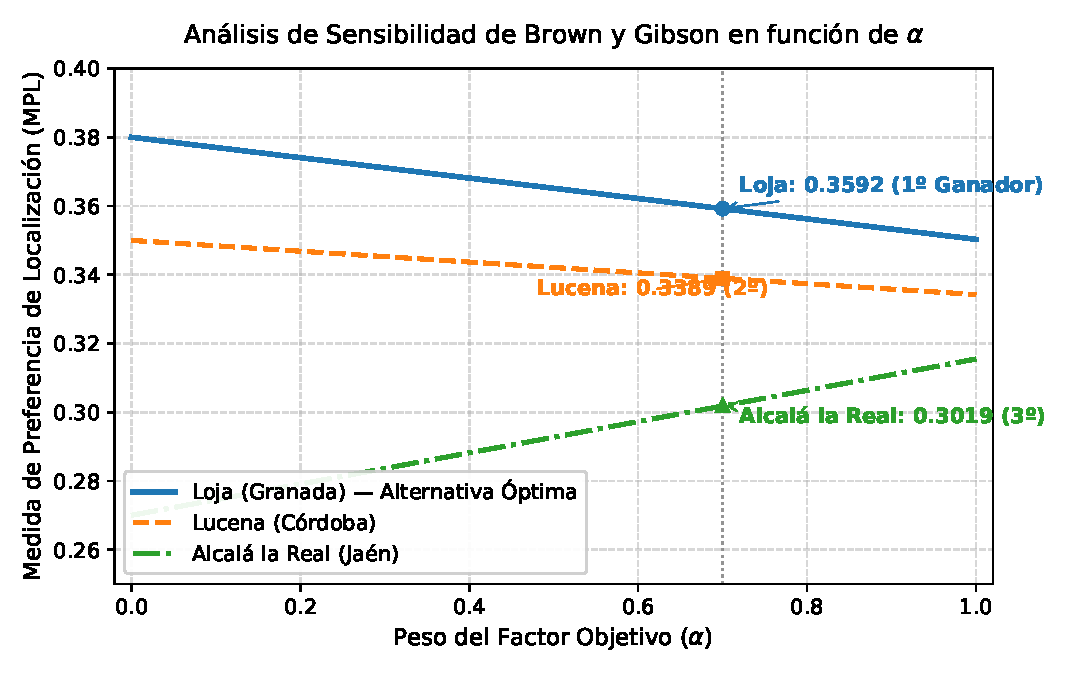
\includegraphics[width=0.92\textwidth]{figuras/sensibilidad_brown_gibson.pdf}
    \caption{Análisis de sensibilidad paramétrico de la Medida de Preferencia de Localización (MPL) según el peso de los factores objetivos ($\alpha$).}
    \label{fig:sensibilidad_bg}
\end{figure}

Como se observa en el gráfico, la curva de \textbf{Loja (El Manzanil~II)} se sitúa estrictamente por encima de Lucena y Alcalá la Real en la totalidad del dominio:
\begin{itemize}
    \item Para $\alpha = 0$ (criterio exclusivamente subjetivo): $MPL_{\text{Loja}} = \num{0.3800} > MPL_{\text{Lucena}} = \num{0.3500} > MPL_{\text{Alcalá}} = \num{0.2700}$.
    \item Para $\alpha = 1$ (criterio exclusivamente económico de costes objetivos): $FO_{\text{Loja}} = \num{0.3503} > FO_{\text{Lucena}} = \num{0.3342} > FO_{\text{Alcalá}} = \num{0.3155}$.
\end{itemize}
En consecuencia, la elección de Loja como ubicación definitiva de la biorrefinería resulta \textbf{robusta, matemáticamente dominante e inmune a variaciones de juicio subjetivo}.

%=============================================================================
\chapter{Cartografía y Planos Justificativos de la Localización}

\section{Marco Normativo y Principios Cartográficos}
Conforme a las exigencias del Seminario 4 y las normas de presentación de proyectos de ingeniería industrial (\textcite{DeCos2008}), la localización definitiva debe justificarse mediante dos niveles cartográficos complementarios:
\begin{enumerate}
    \item \textbf{Plano de Situación (Entorno amplio territorial):} Cartografía oficial a escala normalizada 1:50.000 referenciada al Mapa Topográfico Nacional (MTN50 Hoja 1009, \textit{Loja}) del Instituto Geográfico Nacional (\textcite{IGN2026}), proyectada en el Sistema Geodésico de Referencia oficial en España ETRS89 en el Huso UTM 30N. Representa la inserción territorial, accesos por autovía, nodos de transporte y distancias logísticas hacia centros proveedores y consumidores.
    \item \textbf{Plano de Localización (Entorno próximo parcelario):} Cartografía de detalle a escala normalizada 1:2.000 basada en la información catastral de la Sede Electrónica del Catastro (\textcite{Catastro2026}) y la planimetría urbanística del PGOU de Loja, identificando la parcela industrial, linderos, cotas, viario perimetral y puntos de acometida.
\end{enumerate}

\section{Plano de Situación General (Escala 1:50.000)}
El Plano de Situación (Figura~\ref{fig:plano_situacion}) ilustra la posición estratégica de Loja en el centro neurálgico de Andalucía:
\begin{itemize}
    \item Enlace directo con la autovía A-92 (salida P.K. 187), conectando sin semáforos ni travesías con el Puerto Comercial de Málaga (\SI{68}{\kilo\metre}), centro exportador de lignina y recepción de etanol desnaturalizado.
    \item Comunicación fluida hacia el Corredor Central (Antequera a \SI{45}{\kilo\metre}) y las refinerías de Moeve San Roque (Cádiz) y CLH Cartagena para la expedición del bioetanol 2G.
    \item Radio medio de aprovisionamiento de \SI{35}{\kilo\metre} hacia las \num{42} almazaras del Poniente Granadino (Montefrío, Íllora, Huétor Tájar, Salar, Alhama de Granada).
\end{itemize}

\begin{figure}[H]
    \centering
    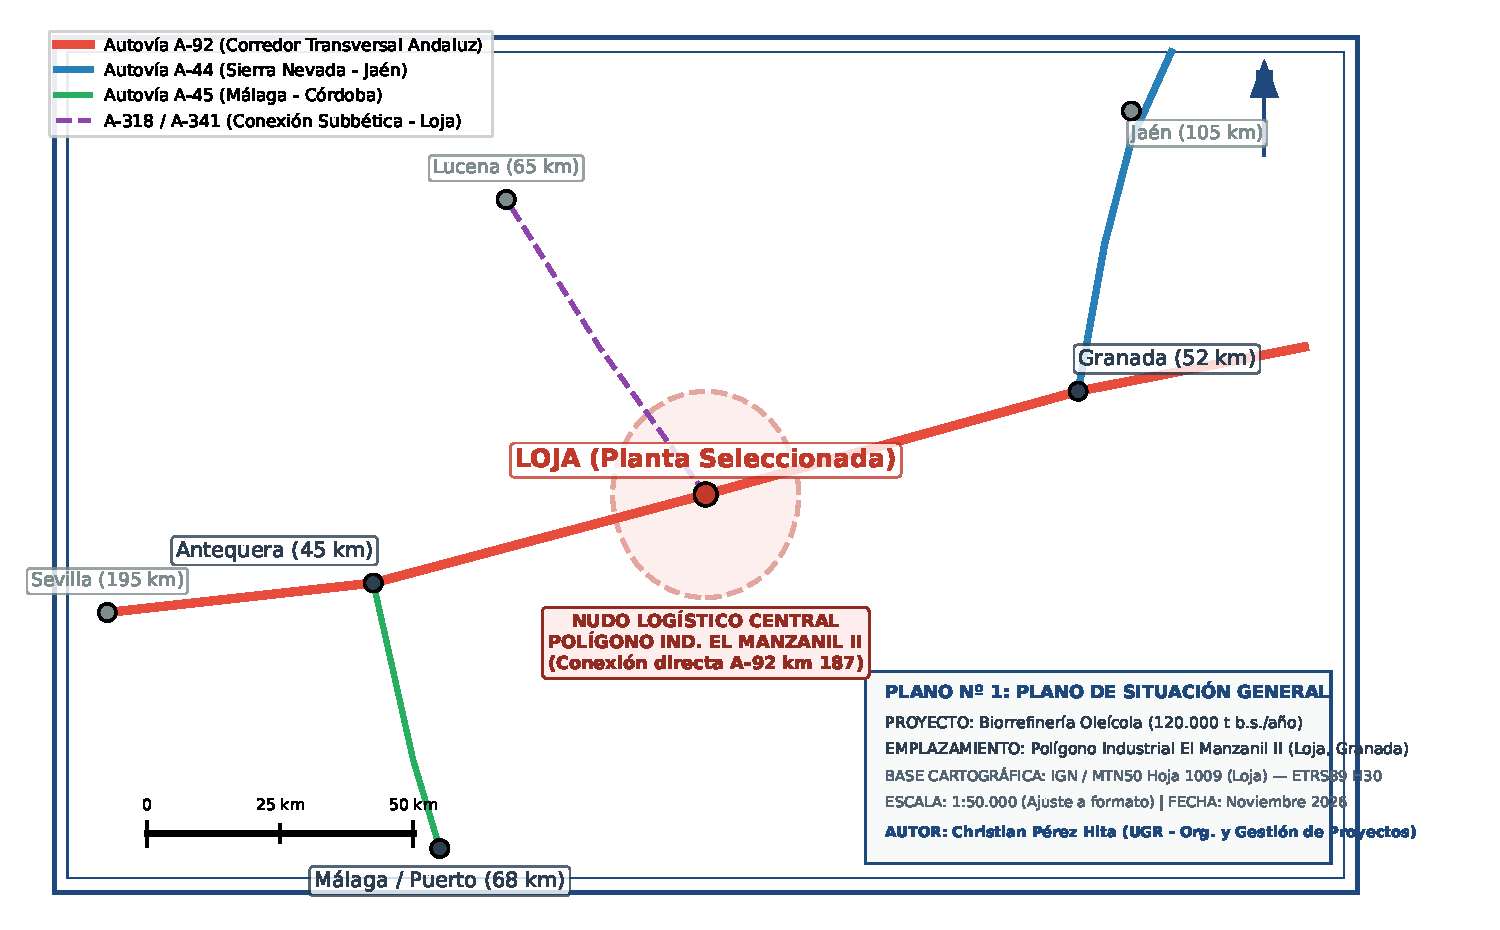
\includegraphics[width=0.98\textwidth]{figuras/plano_situacion.pdf}
    \caption{Plano nº 1: Plano de Situación General (Escala normalizada 1:50.000, Sistema ETRS89 Huso 30). Inserción territorial de la biorrefinería en Loja (Granada) y enlaces viarios principales.}
    \label{fig:plano_situacion}
\end{figure}

\begin{tcolorbox}[colback=blue!5, colframe=blue!60!black, title=Nota Técnica sobre la Cartografía CAD del Proyecto]
El plano vectorial definitivo se encuentra estructurado en el archivo CAD del proyecto (\texttt{F:\textbackslash universidad\textbackslash 4º\textbackslash proyectos\textbackslash Organizacion y gestion de proyectos\textbackslash Planos\_DWG\textbackslash Fatima.dwg}), el cual incorpora el cajetín normalizado (\texttt{Cajetin\_Planos.dwg}), las capas de dibujo topográfico y la rotulación reglamentaria. La Figura~\ref{fig:plano_situacion} presenta la exportación vectorial rasterizada a alta resolución ajustada a formato de memoria técnica.
\end{tcolorbox}

\section{Plano de Localización y Parcela Industrial (Escala 1:2.000)}
El Plano de Localización (Figura~\ref{fig:plano_localizacion}) delimita la parcela seleccionada dentro del Polígono Industrial El Manzanil~II:
\begin{itemize}
    \item \textbf{Referencia de parcela:} Parcela industrial resultante I-14/15, manzana M-3 del Plan Parcial El Manzanil~II.
    \item \textbf{Superficie neta de suelo:} \SI{25000.00}{\square\metre} (\num{2.50} hectáreas).
    \item \textbf{Geometría y dimensiones:} Planta rectangular regular con \SI{125.00}{\metre} de línea de fachada hacia el vial principal sur (Avenida de la Industria) y \SI{200.00}{\metre} de fondo hacia el vial de servicio posterior.
    \item \textbf{Topografía:} Terreno llano acondicionado con pendiente inferior al \SI{1.0}{\percent}, minimizando los movimientos de tierras y terraplenado.
    \item \textbf{Linderos:}
          \begin{itemize}
              \item \textit{Fachada Sur:} Vial Principal (Avenida de la Industria, calzada de \SI{14}{\metre} y aceras de \SI{3}{\metre}).
              \item \textit{Testero Norte:} Parcela I-10 (reserva industrial municipal).
              \item \textit{Lindero Este:} Calle de distribución secundaria y acceso exclusivo a báscula de pesaje de biomasas.
              \item \textit{Lindero Oeste:} Parcela industrial I-16 (industria agroalimentaria compatible).
          \end{itemize}
\end{itemize}

\begin{figure}[H]
    \centering
    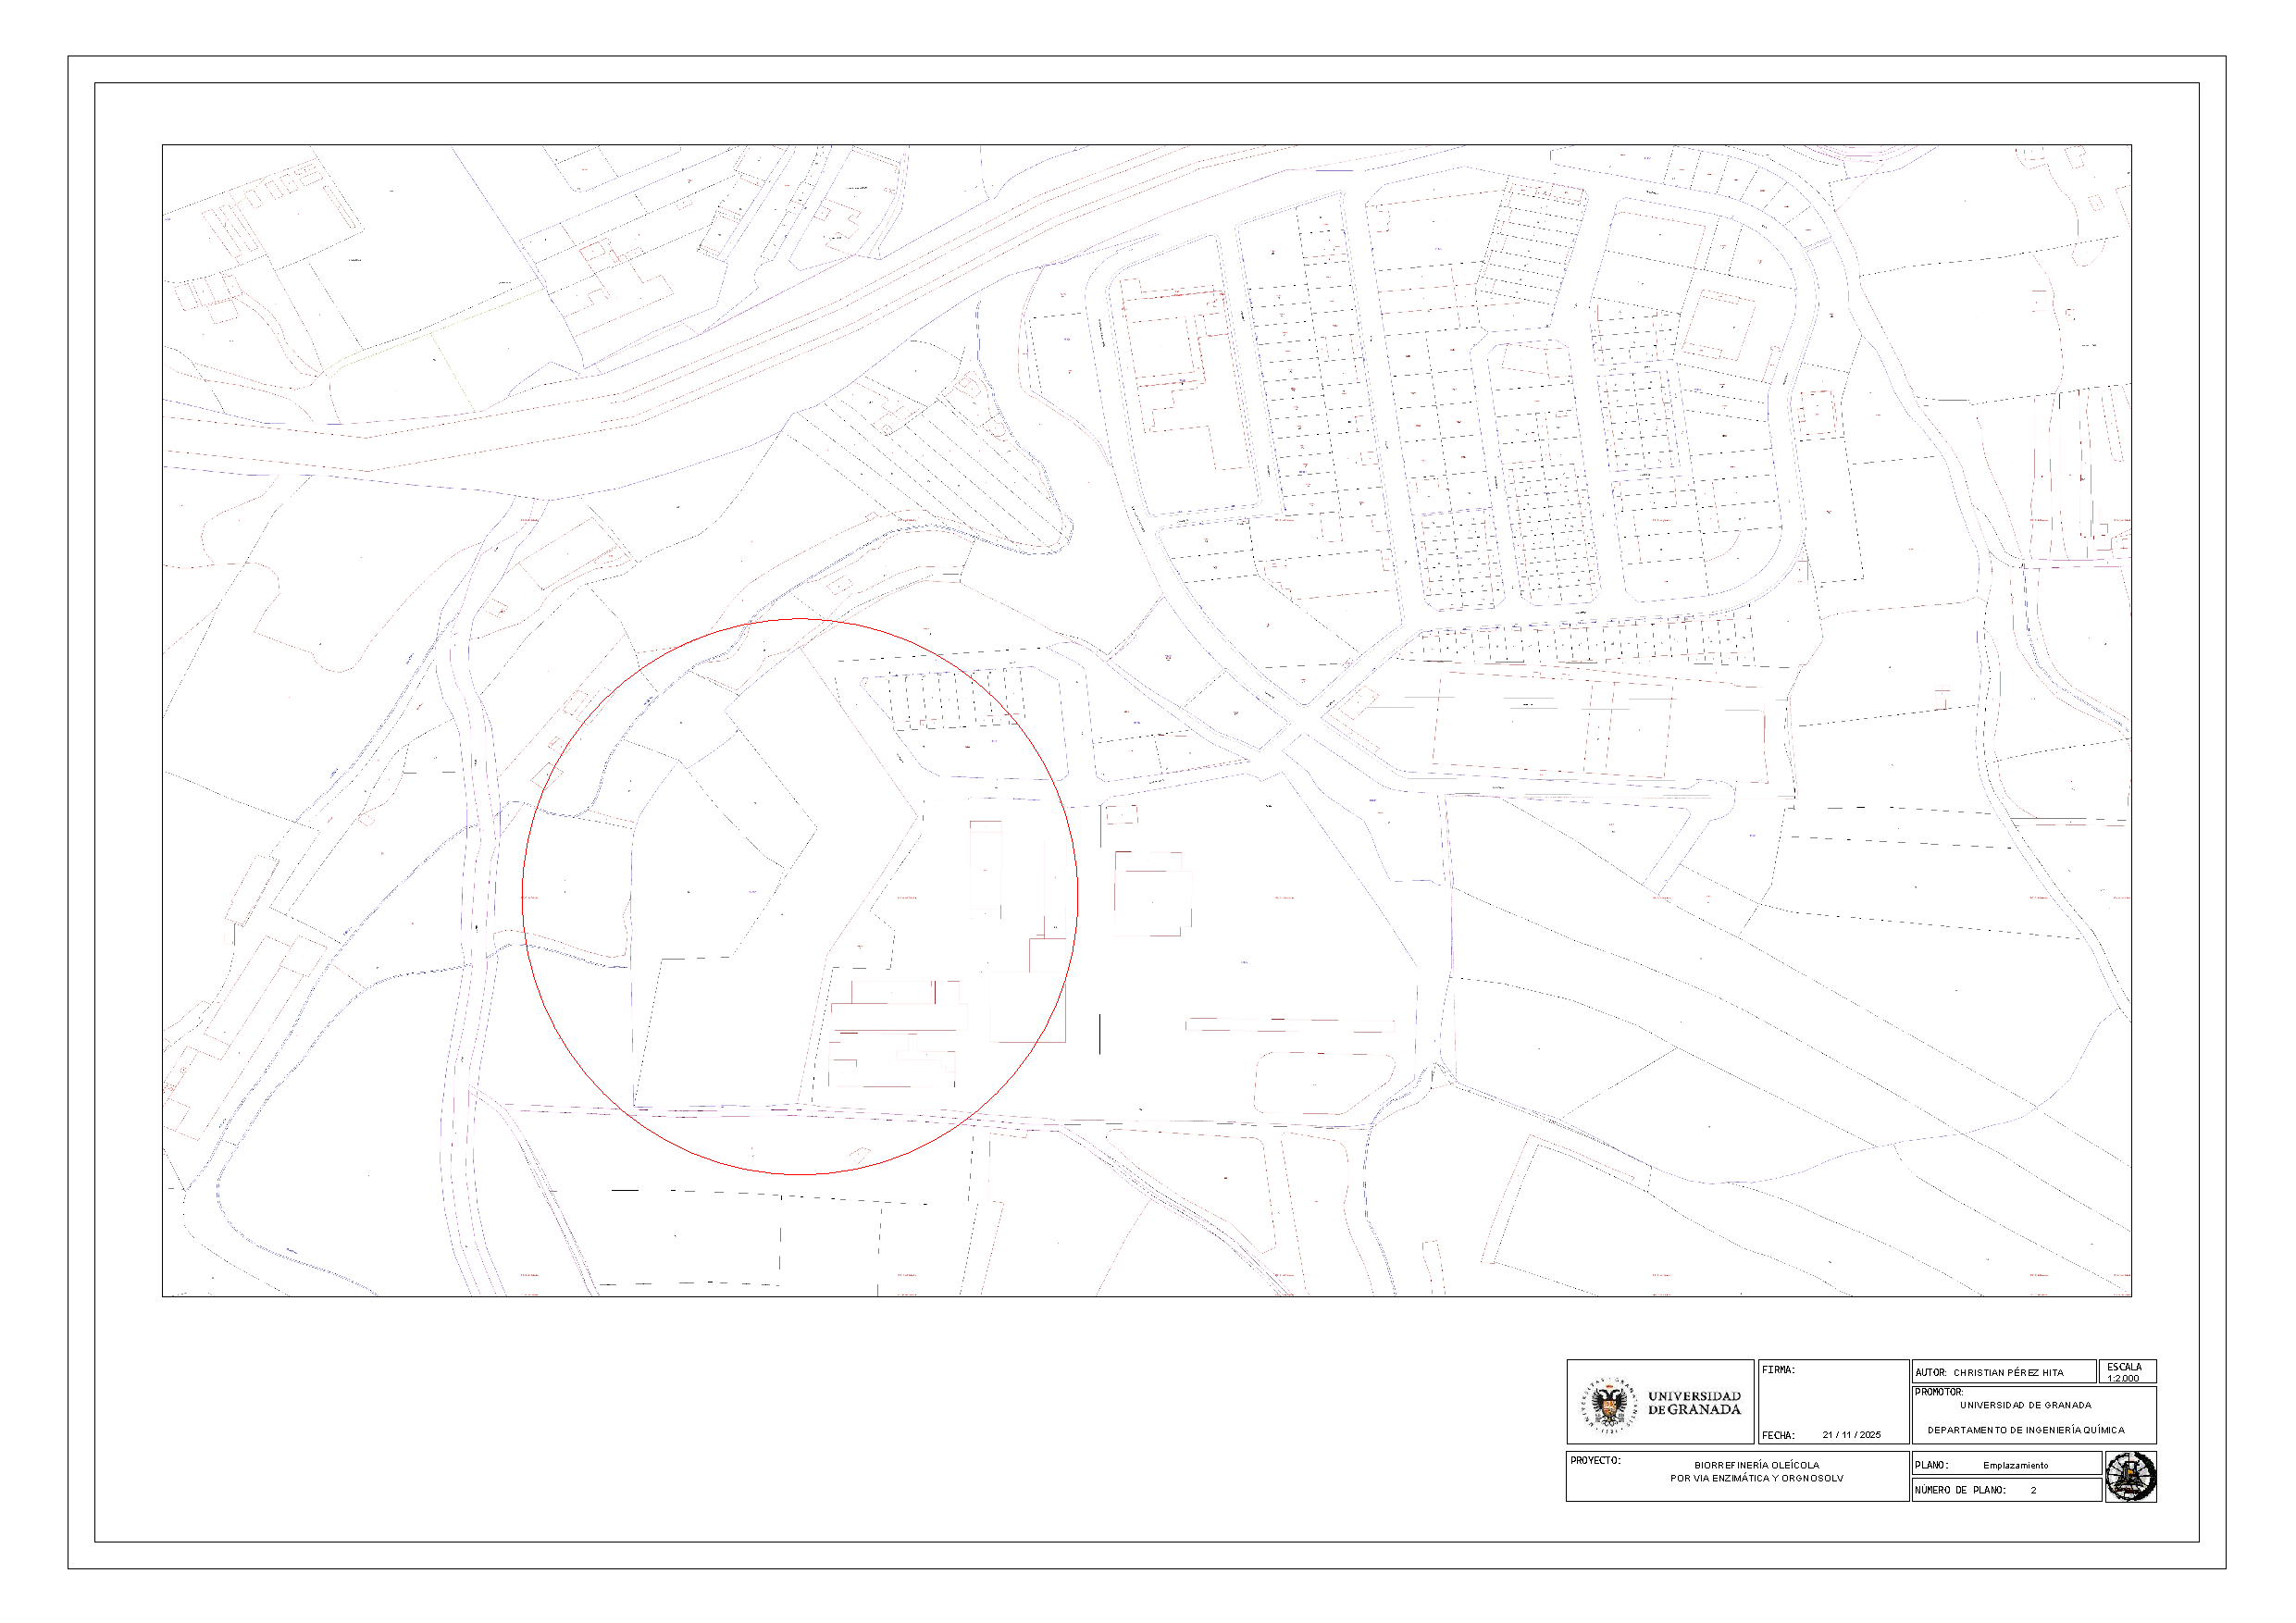
\includegraphics[width=0.98\textwidth]{figuras/plano_localizacion.pdf}
    \caption{Plano nº 2: Plano de Localización y Ordenación General de Parcela (Escala normalizada 1:2.000, Polígono Industrial El Manzanil II, Loja). Delimitación geométrica, retranqueos y accesos segregados.}
    \label{fig:plano_localizacion}
\end{figure}

%=============================================================================
\chapter{Normativa Urbanística, Régimen del Suelo y Acometidas}

\section{Instrumentos de Planeamiento Urbanístico Aplicables}
El suelo donde se emplazará la planta se rige por las determinaciones urbanísticas del \textbf{Plan General de Ordenación Urbana (PGOU) del Excmo. Ayuntamiento de Loja}, aprobado definitivamente mediante Resolución de la Comisión Provincial de Ordenación del Territorio y Urbanismo de Granada, e integrado en el Sistema de Información Territorial y Urbanística de Andalucía (\textcite{SITUA2026}).

La parcela seleccionada se encuentra clasificada como:
\begin{center}
    \textbf{Suelo Urbano Consolidado de Uso Global Industrial, Ordenanza Pormenorizada Grado 2 (Industria Aislada en Gran Parcela).}
\end{center}

\section{Parámetros Urbanísticos y Justificación de Cumplimiento}
La Tabla~\ref{tab:urbanismo} recoge los parámetros urbanísticos de aplicación obligatoria según la ficha urbanística de la manzana M-3 del PGOU de Loja, acreditándose el cumplimiento riguroso de cada índice por parte de la planta biorrefinería proyectada.

\begin{table}[H]
    \centering
    \caption{Comprobación de cumplimiento de las ordenanzas urbanísticas del PGOU de Loja.}
    \label{tab:urbanismo}
    \adjustbox{max width=\textwidth}{%
        \renewcommand{\arraystretch}{1.24}
        \setlength{\tabcolsep}{4.5pt}
        \small
        \begin{tabular}{l c c c}
            \toprule
            \textbf{Parámetro Urbanístico}           & \textbf{Límite PGOU Loja}                 & \textbf{Proyecto Biorrefinería}            & \textbf{Dictamen} \\
            \midrule
            Superficie de parcela neta               & Mínimo \SI{5000}{\square\metre}           & \SI{25000.00}{\square\metre}               & \textbf{Cumple holgadamente} \\
            Longitud de fachada principal            & Mínimo \SI{40.0}{\metre}                  & \SI{125.00}{\metre}                        & \textbf{Cumple} \\
            Coeficiente de edificabilidad neta       & Máximo \SI{1.00}{\square\metre\text{t}/\square\metre\text{s}} & \SI{0.65}{\square\metre\text{t}/\square\metre\text{s}} (\SI{16240}{\square\metre\text{t}}) & \textbf{Cumple} \\
            Ocupación máxima sobre parcela           & Máximo \SI{70.0}{\percent}                & \SI{56.0}{\percent} (\SI{14000}{\square\metre}) & \textbf{Cumple} \\
            Retranqueo a alineación exterior (vial)  & Mínimo \SI{5.00}{\metre}                  & \SI{8.00}{\metre}                          & \textbf{Cumple} \\
            Retranqueo a linderos privados           & Mínimo \SI{3.00}{\metre}                  & \SI{5.00}{\metre}                          & \textbf{Cumple} \\
            Retranqueo a testero posterior           & Mínimo \SI{3.00}{\metre}                  & \SI{6.00}{\metre}                          & \textbf{Cumple} \\
            Altura máxima de cornisa naves           & \SI{12.00}{\metre} (III plantas)          & \SI{10.50}{\metre}                         & \textbf{Cumple} \\
            Elementos técnicos de proceso (Torres)   & Exentos con justificación técnica         & Torres destilación (\SI{24.0}{\metre})     & \textbf{Permitido en art. 8.4} \\
            Reserva de plazas de aparcamiento        & 1 plaza / \SI{100}{\square\metre} const.  & \num{85} plazas interiores                 & \textbf{Cumple} \\
            Reserva de espacios verdes privados      & Mínimo \SI{10.0}{\percent} superficie     & \SI{12.5}{\percent} (\SI{3125}{\square\metre}) & \textbf{Cumple} \\
            \bottomrule
        \end{tabular}%
    }
\end{table}

\section{Dotación de Servicios e Infraestructuras Industriales}
El Polígono El Manzanil~II cuenta con la totalidad de infraestructuras urbanísticas recibidas por el Ayuntamiento de Loja:
\begin{enumerate}
    \item \textbf{Suministro eléctrico en Media y Alta Tensión:}
          \begin{itemize}
              \item Conexión a la línea subterránea de distribución de \SI{20}{\kilo\volt} procedente de la Subestación Transformadora Loja (66/20~kV, Endesa Distribución).
              \item Se proyecta un centro de transformación propio en parcela de \SI{3500}{\kilo\volt\ampere} para alimentar los accionamientos de molienda (\SI{450}{\kilo\watt}), bombeo de reactores (\SI{350}{\kilo\watt}), agitación y servicios auxiliares.
          \end{itemize}
    \item \textbf{Acometida de gas natural:}
          \begin{itemize}
              \item Conexión a la red secundaria MOP 16~bar de Redexis / Enagás que discurre por la Avenida de la Industria.
              \item Suministro auxiliar para la caldera de vapor y arranque del sistema térmico, asegurando una combustión limpia en paralelo al biogás producido en la digestión anaerobia de vinazas.
          \end{itemize}
    \item \textbf{Abastecimiento hídrico industrial:}
          \begin{itemize}
              \item Suministro municipal garantizado mediante tubería de fundición dúctil $\varnothing \SI{200}{\milli\metre}$ con presión manométrica de \SI{4.2}{bar}.
              \item Caudal asignado de hasta \SI{12.0}{\litre/\second}, respaldado por los acuíferos de la Sierra de Loja bajo concesión de la CHG.
          \end{itemize}
    \item \textbf{Saneamiento y Estación Depuradora de Aguas Residuales Industriales (EDARI):}
          \begin{itemize}
              \item Colector general de pluviales y colector de aguas residuales independientes.
              \item La planta dispondrá de una EDARI propia con tratamiento físico-químico primario, balsa de homogenización/neutralización y digestor anaerobio de lodos, garantizando que el efluente final vertido al colector cumpla rigurosamente con los límites de la Ordenanza Municipal de Vertidos de Loja y el Reglamento de Dominio Público Hidráulico.
          \end{itemize}
\end{enumerate}

%=============================================================================
\chapter{Estimación de Mano de Obra Disponible (INE / EPA)}

\section{Requerimientos de Personal de la Planta}
De acuerdo con el dimensionamiento organizativo del proyecto, la biorrefinería requiere una plantilla fija en operación de \textbf{\num{17} trabajadores}, estructurada en los siguientes niveles competenciales:
\begin{itemize}
    \item \textbf{Personal técnico y de gestión cualificado (\num{6} puestos):}
          \begin{itemize}
              \item \num{1} Director de Planta / Ingeniero Químico Responsable.
              \item \num{1} Responsable de Calidad, Seguridad y Medio Ambiente (Químico/Biotecnólogo).
              \item \num{4} Jefes de Turno / Ingenieros Técnicos de Control de Procesos (operación continua $24/7$).
          \end{itemize}
    \item \textbf{Personal de operación y mantenimiento industrial (\num{11} puestos):}
          \begin{itemize}
              \item \num{6} Operadores de planta química (reactores, filtros y tren de destilación).
              \item \num{2} Operadores de parque de biomasas y recepción en báscula.
              \item \num{2} Técnicos especialistas en mantenimiento electromecánico e instrumentación.
              \item \num{1} Operario de almacén y expedición de producto.
          \end{itemize}
\end{itemize}
A este empleo directo se suman más de \num{35} empleos indirectos en el sector del transporte, mantenimiento especializado y cuadrillas de recogida y astillado de poda de olivo en las cooperativas comarcales.

\section{Análisis de Disponibilidad con Datos del INE}
Siguiendo las pautas del Seminario 4 (diapositivas 11--13), se ha consultado la base de datos del \textbf{Instituto Nacional de Estadística (INE)}, específicamente la *Encuesta de Población Activa (EPA)* y las estadísticas del Mercado Laboral comarcal (\textcite{INE2025}):
\begin{enumerate}
    \item \textbf{Mano de obra altamente cualificada (Titulados universitarios):}
          \begin{itemize}
              \item La cercanía a la ciudad de Granada (\SI{52}{\kilo\metre}, \num{35} minutos directos por autovía A-92) garantiza un acceso inmejorable a los egresados de la \textbf{Universidad de Granada (UGR)}, una de las principales instituciones académicas de España en Ingeniería Química, Biotecnología y Química.
              \item No se requiere la reubicación forzosa de personal directivo ni sobrecostes de expatriación, posibilitando la atracción y fidelización de talento técnico especializado en procesos de fermentación y catálisis.
          \end{itemize}
    \item \textbf{Mano de obra técnica y operaria local:}
          \begin{itemize}
              \item Loja y las cabeceras comarcales limítrofes (Huétor Tájar, Antequera, Lucena) cuentan con centros de Formación Profesional reglada que imparten ciclos formativos de Grado Medio y Superior en:
                    \begin{itemize}
                        \item *Mantenimiento Electromecánico y Mecatrónica Industrial*.
                        \item *Automatización y Robótica Industrial*.
                        \item *Laboratorio de Análisis y Control de Calidad*.
                    \end{itemize}
              \item La EPA refleja una tasa de paro comarcal en el Poniente Granadino del \SI{18.4}{\percent}, con un significativo excedente de población activa joven con formación técnica que demanda empleo estable en el sector industrial, superando la precariedad de la estacionalidad agrícola.
              \item El Ayuntamiento de Loja y el Servicio Andaluz de Empleo (SAE) contemplan convenios de formación a medida para operarios industriales de nueva implantación con bonificaciones en la cotización a la Seguridad Social.
          \end{itemize}
\end{enumerate}

%=============================================================================
\chapter{Bases para la Implantación de la Planta (Layout y Espacios)}

\section{Metodología de Distribución en Planta (SLP de Muther)}
Para la ordenación espacial de la parcela se aplica la metodología de \textbf{Distribución Sistemática de las Instalaciones (\textit{Systematic Layout Planning}, SLP)} formulada por Richard Muther (\textcite{MeyersStephens2005}). El método busca minimizar los costes de manipulación y transporte interno de materiales, optimizar la seguridad operacional y garantizar circulaciones fluidas y sin interferencias entre zonas limpias y áreas de proceso pesado.

\section{Definición de Áreas Funcionales y Actividades}
La planta se descompone en las siguientes \num{10} áreas funcionales principales:
\begin{enumerate}
    \item \textbf{Área 1: Recepción, Báscula y Control de Accesos (\SI{800}{\square\metre}):} Garita de seguridad, báscula puente de pesaje de camiones de \SI{60}{\tonne} y toma de muestras de biomasa para análisis de humedad.
    \item \textbf{Área 2: Parque de Biomasas y Almacenamiento (\SI{4800}{\square\metre}):} Silos verticales cerrados para \SI{3000}{\tonne} de hueso de aceituna, parque exterior pavimentado para almacenamiento y astillado de leña de poda, y fosa cubierta de descarga de hoja.
    \item \textbf{Área 3: Nave de Preparación Mecánica (\SI{1600}{\square\metre}):} Secador rotatorio indirecto por gases limpios de combustión, molino triturador de martillos y tamiz clasificatorio rotativo con ciclones de aspiración de polvo.
    \item \textbf{Área 4: Nave de Proceso Químico y Biológico (\SI{5200}{\square\metre}):} Batería de reactores tubulares de hidrólisis ácida previa, reactor presurizado Organosolv, cámara flash de despresurización, filtros de banda, biorreactores continuos de fermentación de pentosas (C5) y tren de sacarificación y fermentación simultánea (SSF C6).
    \item \textbf{Área 5: Tren de Destilación y Parque de Tanques (\SI{1600}{\square\metre}):} Columnas de fraccionamiento y rectificación hidroalcohólica en intemperie (\SI{24}{\metre} de altura), columna de desorción de solventes, condensadores y cubeto estanco con tanques aéreos de almacenamiento de bioetanol comercial, etanol absoluto desnaturalizado y furfural.
    \item \textbf{Área 6: Almacén de Lignina, Biofertilizante y Expedición (\SI{3840}{\square\metre}):} Nave climatizada para secado, ensacado y paletizado de lignina técnica pura de alta pureza (\textcite{RomeroGarcia2022}), almacenamiento de biofertilizante estabilizado y muelles de carga cubiertos para camiones de expedición.
    \item \textbf{Área 7: Planta de Tratamiento de Efluentes (EDARI) y Biogás (\SI{2400}{\square\metre}):} Digestor anaerobio de vinazas residuales para generación de biometano, balsa de aireación y deshidratación centrífuga de lodos.
    \item \textbf{Área 8: Generación Térmica y Servicios Auxiliares (\SI{1800}{\square\metre}):} Caldera acuotubular de vapor de cogeneración alimentada por biogás/fracción pesada, torres de refrigeración de circuito cerrado, compresores de aire de control y subestación eléctrica de \SI{3.5}{\mega\volt\ampere}.
    \item \textbf{Área 9: Edificio de Laboratorio, I+D y Sala de Control (\SI{1200}{\square\metre}):} Sala de control con sistema distribuido DCS/SCADA, laboratorio físico-químico y microbiológico de control de fermentaciones y cromatografía.
    \item \textbf{Área 10: Edificio Administrativo, Vestuarios y Aparcamientos (\SI{1760}{\square\metre}):} Oficinas generales de dirección y compras, vestuarios de personal de planta, comedor social y aparcamiento exterior pavimentado de \num{85} plazas.
\end{enumerate}

\section{Matriz de Relaciones de Proximidad (Matriz de Muther)}
Siguiendo la metodología SLP, se establecen los códigos de proximidad normalizados entre cada par de actividades:
\begin{itemize}
    \item \textbf{A (Absolutamente necesario):} Proximidad crítica por flujo masivo de materia o tubería compartida.
    \item \textbf{E (Especialmente importante):} Flujo regular de personal o intercambio energético directo.
    \item \textbf{I (Importante):} Conveniencia operativa y compartición de servicios auxiliares.
    \item \textbf{O (Ordinario):} Relación estándar sin condicionantes severos.
    \item \textbf{U (Sin importancia):} Ausencia de interrelación funcional o espacial.
    \item \textbf{X (No deseable):} Incompatibilidad estricta por riesgo de explosión ATEX, contaminación cruzada, ruidos o emisión de polvo.
\end{itemize}

\begin{table}[H]
    \centering
    \caption{Matriz de Interrelación de Actividades y Espacios (Metodología SLP).}
    \label{tab:matriz_slp}
    \adjustbox{max width=\textwidth}{%
        \renewcommand{\arraystretch}{1.24}
        \setlength{\tabcolsep}{4.0pt}
        \small
        \begin{tabular}{l cccccccccc}
            \toprule
            \textbf{Actividad / Área Funcional} & \textbf{1} & \textbf{2} & \textbf{3} & \textbf{4} & \textbf{5} & \textbf{6} & \textbf{7} & \textbf{8} & \textbf{9} & \textbf{10} \\
            \midrule
            1. Recepción, Báscula y Accesos     & --         & A          & U          & U          & U          & E          & U          & U          & O          & I           \\
            2. Parque y Silos de Biomasas       &            & --         & A          & U          & X          & U          & U          & I          & X          & X           \\
            3. Nave de Preparación Mecánica     &            &            & --         & A          & X          & U          & U          & I          & X          & X           \\
            4. Nave de Proceso Químico          &            &            &            & --         & A          & I          & A          & E          & I          & U           \\
            5. Tren Destilación y Tanques (ATEX)&            &            &            &            & --         & I          & E          & E          & I          & X           \\
            6. Almacén de Lignina y Expedición  &            &            &            &            &            & --         & U          & U          & O          & I           \\
            7. Depuración EDARI y Biogás        &            &            &            &            &            &            & --         & A          & U          & X           \\
            8. Servicios Auxiliares y Caldera   &            &            &            &            &            &            &            & --         & I          & O           \\
            9. Laboratorio y Sala de Control    &            &            &            &            &            &            &            &            & --         & E           \\
            10. Oficinas, Social y Aparcamiento &            &            &            &            &            &            &            &            &            & --          \\
            \bottomrule
        \end{tabular}%
    }
\end{table}

\section{Directrices de Circulación e Implantación en Parcela}
De la matriz SLP se desprenden los principios rectores aplicados en el Plano de Localización (Figura~\ref{fig:plano_localizacion}):
\begin{enumerate}
    \item \textbf{Segregación estricta de tráficos:} El tráfico pesado de camiones bañera (biomasa) y camiones cisterna (solventes y bioetanol) ingresa exclusivamente por el vial lateral este, dirigiéndose a la báscula y parque de biomasas sin cruzarse jamás con los turismos del personal o visitas, los cuales acceden directamente por el vial sur hacia el aparcamiento frontal.
    \item \textbf{Aislamiento de áreas ATEX:} El parque de tanques y la torre de destilación fraccionada se sitúan en el cuadrante este de la parcela, respetando las distancias de seguridad reglamentarias del Real Decreto 656/2017 (Reglamento APQ) y apartadas de focos de ignición y de los edificios de oficinas.
    \item \textbf{Orientación respecto a vientos dominantes:} Los vientos dominantes en Loja (componente Oeste--Suroeste) barren la parcela de izquierda a derecha. Por ello, el parque de biomasas y la nave de molienda se ubican a sotavento del edificio administrativo y laboratorios, impidiendo que el polvo en suspensión alcance las áreas sociales.
    \item \textbf{Circuito cerrado de energía y vinazas:} La proximidad adyacente entre la EDARI (Área 7) y la caldera de vapor (Área 8) optimiza la tubería de biometano depurado para autoconsumo térmico directo, minimizando las pérdidas de carga y garantizando la sostenibilidad circular de la planta.
\end{enumerate}

%=============================================================================
\chapter{Conclusiones y Juicio Técnico del Autor}

\section{Conclusiones Principales del Estudio}
El desarrollo del estudio de localización e implantación para la biorrefinería oleícola de \SI{120000}{\tonne\text{ b.s.}/a\text{\~{n}}o} permite formular las siguientes conclusiones técnicas:
\begin{enumerate}
    \item \textbf{Idoneidad macrolocal de Granada y el Poniente Granadino:} La investigación empírica a partir de balances de AICA y datos empresariales de SABI demuestra que, a pesar de que Jaén posee la mayor masa bruta de olivar, la alta densidad de orujeras convencionales genera un mercado saturado con precios del hueso muy elevados. El Poniente Granadino ofrece un ratio de oportunidad de \textbf{128,47~M€/competidor}, asegurando la adquisición de las \SI{120000}{\tonne\text{ b.s.}/a\text{\~{n}}o} con costes de flete mínimos en un radio medio de \SI{35}{\kilo\metre}.
    \item \textbf{Preferencia incontestable de Loja (Polígono El Manzanil~II):} La aplicación rigurosa del método de Brown y Gibson dictamina que el Polígono Industrial El Manzanil~II en Loja es la alternativa más eficiente, con un índice de preferencia global $MPL = \num{0.3592}$ (frente a \num{0.3389} en Lucena y \num{0.3019} en Alcalá la Real). El análisis de sensibilidad ratifica que Loja es la solución óptima para cualquier valor del factor de coste $\alpha \in [0, 1]$.
    \item \textbf{Viabilidad urbanística y suficiencia de parcela:} La parcela seleccionada (Parcela I-14/15 con \SI{25000}{\square\metre}) cumple de forma holgada todas las prescripciones del PGOU de Loja para suelo industrial consolidado Grado 2: ocupación del \SI{56}{\percent} (inferior al límite del \SI{70}{\percent}), edificabilidad de \SI{0.65}{\square\metre\text{t}/\square\metre\text{s}} (frente a \num{1.00} admisible) y retranqueos reglamentarios respetados en todos sus linderos.
    \item \textbf{Disponibilidad de infraestructuras y mano de obra:} El emplazamiento dispone de acometida eléctrica de 20~kV en el propio polígono, red de gas natural MOP 16~bar y abastecimiento de agua de la CHG. La cercanía inmediata a la Universidad de Granada (a 35 minutos por A-92) garantiza el reclutamiento directo de ingenieros químicos y personal de laboratorio, mientras que los ciclos de Formación Profesional de Loja cubren plenamente los perfiles de mantenimiento electromecánico y operación continua.
    \item \textbf{Distribución funcional optimizada:} La ordenación de la parcela según el método SLP de Muther asegura circulaciones seguras, segregación estricta del tráfico pesado de biomasas respecto al tráfico de turismos y cumplimiento exhaustivo de las distancias de seguridad APQ y normativa ATEX.
\end{enumerate}

\section{Recomendaciones para las Fases Posteriores del Proyecto}
Con vistas a la redacción del proyecto de detalle y la integración definitiva de los planos de ingeniería en AutoCAD (\texttt{Planos\_DWG/Fatima.dwg}):
\begin{itemize}
    \item Solicitar formalmente al Ayuntamiento de Loja la cédula urbanística informativa previa de la Parcela I-14/15 y la reserva de potencia eléctrica de 3,5 MVA ante Endesa Distribución.
    \item Iniciar los trámites de Autorización Ambiental Integrada (AAI) ante la Delegación Territorial de Sostenibilidad, Medio Ambiente y Economía Azul de la Junta de Andalucía en Granada.
    \item Suscribir acuerdos marco de pre-contrato de suministro (\textit{offtake agreements}) con las principales cooperativas almazareras del Poniente Granadino (Loja, Huétor Tájar, Montefrío e Íllora) durante el primer semestre previo al inicio de las obras.
\end{itemize}

\vspace{3.5em}
\noindent\begin{tabular*}{\linewidth}{@{}l @{\extracolsep{\fill}} r@{}}
\textbf{Firma del Estudiante:} & \textbf{Fecha:} 03/11/2026 \\[0.4em]
\hline
\rule{0pt}{1.4em}Christian Pérez Hita &
\end{tabular*}

%=============================================================================
\printbibliography[heading=bibintoc, title={Referencias Bibliográficas}]

\end{document}
